%%%%%%%%%%%%%%%%%%%%%%%%%%%%%%%%%%%%%%%%%%%%%%%%%%%%%%%%%%
% Formattazione base del documento con supporto caratteri
% accentati da tastiera win/linux e lingua italiana
%%%%%%%%%%%%%%%%%%%%%%%%%%%%%%%%%%%%%%%%%%%%%%%%%%%%%%%%%%

\documentclass[12pt,a4paper,oneside,openright]{book}
%modifico l'interlinea
\linespread{1.3}


\usepackage[utf8]{inputenc}
\usepackage[italian]{babel}

%%%%%%%%%%%%%%%%%%%%%%%%%%%%%%%%%%%%%%%%%%%%%%%%%%%%%%%%%%%%
% Pacchetto per il controllo della sintassi
% Decommentare \syntaxonly
%%%%%%%%%%%%%%%%%%%%%%%%%%%%%%%%%%%%%%%%%%%%%%%%%%%%%%%%%%

\usepackage{syntonly}
\usepackage{textcomp}
%\usepackage{dsfont}
% \syntaxonly

%%%%%%%%%%%%%%%%%%%%%%%%%%%%%%%%%%%%%%%%%%%%%%%%%%%%%%%%%%
% Inclusione pacchetto per la gestione delle figure che
% andranno copiate nella cartella figure
%
% Esempio di uso: avendo un file di nome figura1.eps questa
% si inserisce nella tesi con il comando:
%
% \begin{figure}[ht]
% \begin{center}
% \includegraphics{figura1.eps}
% \caption[nome breve]{nome lungo}
% \end{center}
% \end{figure}
%
% Il nome breve è quello che apparirà nell'indice delle
% figure ed è opzionale.
% Il nome lungo è quello che appare sotto la figura.
%%%%%%%%%%%%%%%%%%%%%%%%%%%%%%%%%%%%%%%%%%%%%%%%%%%%%%%%%%

\usepackage[final]{graphicx}
%\graphicspath{{./images/}}
\DeclareGraphicsExtensions{.png,.pdf,.jpg}

% evita il warning di pdllatex riguardo alle immagini pdf
% con versione 1.5 (al massimo 1.4 era di default..)
\pdfoptionpdfminorversion=5

% small 
\usepackage[font=small]{caption}

%\usepackage{subfigure}
%\usepackage{wrapfig}


%%%%%%%%%%%%%%%%%%%%%%%%%%%%%%%%%%%%%%%%%%%%%%%%%%%%%%%%%%
% Inclusione pacchetto per la generazione automatica
% dell'indice analitico.  Per esempio se vogliamo che la
% parola "raggruppamenti" sia indicizzata nella frase
% "I raggruppamenti sono realizzati per..." si dovrà
% scrivere "i raggruppamenti\index{raggruppamenti} ..."
%
% Compilando il file, il LaTeX produrrà un file ausiliario
% che termina con ".idx". Bisogna far processare questo
% file idx dal programma ausiliario "bibtex", che produrrâ
% a sua volta un altro file ancora. Dare infine un'ultima
% passata col LaTeX. Si può tranquillamente lasciare la
% compilazione dell'indice verso la fine della stesura del
% lavoro, quando tutto è ormai quasi definitivo.
%%%%%%%%%%%%%%%%%%%%%%%%%%%%%%%%%%%%%%%%%%%%%%%%%%%%%%%%%%

%\usepackage{makeidx}
%\usepackage{tocbibind}
%\makeindex

%%%%%%%%%%%%%%%%%%%%%%%%%%%%%%%%%%%%%%%%%%%%%%%%%%%%%%%%%%
% Numerazione delle sessioni fino alle subsub e inclusione
% nell'indice
%%%%%%%%%%%%%%%%%%%%%%%%%%%%%%%%%%%%%%%%%%%%%%%%%%%%%%%%%%

%\setcounter{secnumdepth}{4}
\setcounter{tocdepth}{4}

%%%%%%%%%%%%%%%%%%%%%%%%%%%%%%%%%%%%%%%%%%%%%%%%%%%%%%%%%%
% Inclusione pacchetto per la gestione della impostazioni
% personalizzate per la prima pagina
%%%%%%%%%%%%%%%%%%%%%%%%%%%%%%%%%%%%%%%%%%%%%%%%%%%%%%%%%%

\usepackage{unipr}
    \titolo{Trasferimento dell'attenzione in reti GAN cicliche}
    \titoloIng{Attention transfer for cycle consistent generative adversarial networks}
    \laureando{Filippo Botti matr. 287065}
    \annoaccademico{2019-2020}
    \corsodilaurea{Ingegneria Informatica, Elettronica e delle Telecomunicazioni}
    \relatore[Chiar.mo Prof.]{Andrea Prati}
    \correlatorea[Ing.]{Tomaso Fontanini}
    \dedica{Ai miei genitori.}
    \citazione{\textit{\textquotedblleft Se ho visto più lontano, \`e perch\`e stavo sulle spalle di giganti.\textquotedblright \\
	Isaac Newton }}


%%%%%%%%%%%%%%%%%%%%%%%%%%%%%%%%%%%%%%%%%%%%%%%%%%%%%%%%%%
% utilizzo il pacchetto fancyhdr per l'header e il footer
%%%%%%%%%%%%%%%%%%%%%%%%%%%%%%%%%%%%%%%%%%%%%%%%%%%%%%%%%%

\usepackage{fancyhdr}


 % Package aggiunti
  \usepackage{amssymb}				% matematica
  \usepackage{amsmath}				% matematica
  \usepackage{amsthm}				% matematica -> stile teoremi, def, proposizioni
  \usepackage{amsbsy}				% for bold math symbol
  \usepackage{cases}				% sistemi di equazioni con numerazione e sottonumerazione
  \usepackage{booktabs}				% tabelle con toprule ecc
  \usepackage{textcomp}				% per il simbolo di gradi
  \usepackage{subfig}				% per mettere pi figure in una stessa
  \usepackage{minted}
 \usepackage[dvipsnames]{xcolor}
\definecolor{lightGray}{RGB}{236,236,236}
  \usepackage[chapter]{algorithm}	% per mettere l'ambiente flottante attorno all'algoritmo (chapter \`e per la numerazione)
  \usepackage{algorithmic}			% per creare algoritmi
  \floatname{algorithm}{Algoritmo}					% opzioni dell'algoritmo: titolo in italiano
  \renewcommand{\algorithmicrequire}{\textbf{Input:}}		% require->input
  \renewcommand{\algorithmicensure}{\textbf{Output:}}	% ensure->output
  \setlength{\parindent}{0in}			% per togliere l'indentazione all'inizio di un nuovo paragrafo

%%%%%%%%%%%%%%%%%%%%%%%%%%%%%%%%%%%%%%%%%%%%%%%%%%%%%%%%%%
% utilizzo il pacchetto hyperref per i link nel pdf, oltretutto setto i colori dei link a nero
% nota: funziona solo con pdfLatex
%%%%%%%%%%%%%%%%%%%%%%%%%%%%%%%%%%%%%%%%%%%%%%%%%%%%%%%%%%

\usepackage[pdftex,colorlinks,plainpages=false,hyperindex,bookmarksopen,linkcolor=black,citecolor=black,urlcolor=black]{hyperref}
% pacchetto per creare i link con pdfLatex
%\usepackag{hyperref}
%\hypersetup{colorlinks=true, linkcolor=black, urlcolor=black}

%%%%%%%%%%%%%%%%%%%%%%%%%%%%%%%%%%%%%%%%%%%%%%%%%%%%%%%%%%
% Comandi aggiuntivi
%%%%%%%%%%%%%%%%%%%%%%%%%%%%%%%%%%%%%%%%%%%%%%%%%%%%%%%%%%
\newcommand{\EQ}[1]{Eq.~(\ref{#1})}
\newcommand{\BEGMATRIX}[1]{\left[\begin{array}{#1}}
\newcommand{\ENDMATRIX}{\end{array}\right]}
\def\argmin{\mathop{\rm argmin}}

%%%%%%%%%%%%%%%%%%%%%%%%%%%%%%%%%%%%%%%%%%%%%%%%%%%%%%%%%%
% Corpo della tesi
%%%%%%%%%%%%%%%%%%%%%%%%%%%%%%%%%%%%%%%%%%%%%%%%%%%%%%%%%%

\begin{document}

% PAGE HEADERS permette di creare gli header delle pagine con il numero, il capitolo e la riga sotto
\pagestyle{fancy}
\headheight 15pt
\renewcommand{\chaptermark}[1]{\markboth{{\chaptername}\ \thechapter.\hspace{1em}#1}{}}
\renewcommand{\footrulewidth}{0pt}
% definisce l'header e il footer
\lhead[\fancyplain{}{}]{\fancyplain{}{\leftmark}} \chead{}
\rhead{\thepage} \lfoot{} \cfoot{} \rfoot{}

% definizione dei teoremi, proposizioni, definizioni ecc usato con il package amsthm
%	\newtheorem{definizione}{Definizione}[chapter] 		% il chapter si usa per la sotto numerazione nei capitoli
%	\newtheorem{proposizione}{Proposizione}[chapter]
%	\newtheorem{problema}{Problema}[chapter]
%	\newtheorem{proprieta}{Propriet\`a}[chapter]


%%%%%%%%%%%%%%%%%%%%%%%%%%%%%%%%%%%%%%%%%%%%%%%%%%%%%%%%%%
% Inizio della parte introduttiva
%%%%%%%%%%%%%%%%%%%%%%%%%%%%%%%%%%%%%%%%%%%%%%%%%%%%%%%%%%

\frontmatter
\pagenumbering{alph}
\maketitle
\chapter*{Ringraziamenti}


\pagenumbering{roman}
\tableofcontents
%\listoffigures




%\lstlistoflistings


%%%%%%%%%%%%%%%%%%%%%%%%%%%%%%%%%%%%%%%%%%%%%%%%%%%%%%%%%%
% Inizio della parte centrale
%%%%%%%%%%%%%%%%%%%%%%%%%%%%%%%%%%%%%%%%%%%%%%%%%%%%%%%%%%
% \pagenumbering{arabic}
\mainmatter
         \chapter*{Introduzione} % \chapter* -> the introduction isn't the Chapter 1, it's not a numbered chapter
\addcontentsline{toc}{chapter}{Introduzione} %this line enable the introduction to be listed in the Table Of Contents even if it's not a numbered chapter (see above)


 \clearpage
         \chapter{Stato dell'arte}
Illustriamo ora lo stato dell'arte relativo alle Cycle Generative Adversarial Networks (GAN), delle reti di Deep Learning in grado di tradurre immagini da un insieme ad un altro. Verranno analizzate le architetture sulle quali si basano queste reti e i concetti teorici che le caratterizzano. Inoltre verrà trattato un algoritmo per la rappresentazione visiva di come agiscono queste reti: GradCam.

\section{Machine Learning}
\emph{
    \textquotedblleft Si dice che un programma apprende dall'esperienza E con riferimento a alcune classi di compiti T e con misurazione della performance P, se le sue performance nel compito T, come misurato da P, migliorano con l'esperienza E.\textquotedblright
}
    \begin{flushright}
        \emph{Tom Mitchell \cite{tom1997hill}}
    \end{flushright}
Il Machine Learning è una branca dell'intelligenza artificiale che basa il suo funzionamento sulla capacità di apprendere dai dati e dalle esperienze passate \cite{mohri2018foundations}.
Sostanzialmente il Machine Learning cerca di insegnare ai computer a comportarsi come gli esseri umani: imparando dall'esperienza. Esso infatti non è altro che un metodo di analisi dei dati automatizzato che preso un set di dati in ingresso è in grado di effettuare una previsione su di esso basandosi su un modello.
Per capire meglio il concetto aiutiamoci con un esempio: supponiamo di dover creare un sistema in grado di rilevare la presenza di un cavallo all'interno di un'immagine. Questo compito, svolto da un essere umano dotato di pensiero, è un compito molto semplice: il nostro cervello sa com'è fatta la fisionomia di un cavallo, non deve far altro che confrontare l'immagine che vede con ciò che ricorda ed infine stabilire se è conforme o meno. Ora, supponiamo di voler sostituire l'essere umano con un computer, come facciamo a programmare una macchina per distringuere una foto con un cavallo rispetto a qualsiasi altra foto? L'idea è, appunto, quella di utilizzare un algoritmo di Machine Learning per addestrare il computer a rilevare l'animale. Rimanendo sull'analogia tra essere umano e computer, possiamo sfruttare il ragionamento di base dell'uomo e riportarlo sulla macchina: possiamo mostrare al computer tante immagini di cavalli come esempi, per far si che impari a riconoscerli. Per insegnargli a riconoscerle dovremo definire un insieme di parametri, detti features, utili al riconoscimento del cavallo. Possiamo, ad esempio, dire al computer di verificare la fisionomia delle orecchie, il colore del manto e la presenza o meno della criniera. Dovremo quindi verificare la presenza di tutti questi tratti e, infine, potremo determinare, con un margine di errore, se la foto in questione ritrae o meno un cavallo.

\subsection{Addestramento e discesa del gradiente}
Andando più nel dettaglio, possiamo dire che, dato un insieme in ingresso $X$ composto dagli esempi e dalle features che il modello deve estrarre e un insieme in uscita $Y$, composto dai valori che l'uscita può assumere (1 se presente il cavallo oppure 0, nel nostro caso di esempio), stiamo cercando una funzione $f(x)$ tale per cui: $$f(x): X \rightarrow Y$$
ovvero un'applicazione che associ ai valori $x$ un'uscita $y$.
\\Per ricavare l'applicazione cercata dovremo associare dei pesi $w$ alle features, tali per cui: $$y = w\textsubscript{1}x\textsubscript{1} + w\textsubscript{2}x\textsubscript{2} + ... +
w\textsubscript{n}x\textsubscript{n}$$ 
Dobbiamo quindi trovare il valore ottimo dei pesi in questione e lo facciamo attraverso l'addestramento della rete: partendo con pesi dal valore casuale, per ogni esempio, calcoliamo l'uscita $y$ e la confrontiamo con il valore associato all'esempio, al fine di calcolare la funzione d'errore (che ci indica, per l'appunto, quanto siamo distanti dal valore corretto). Una volta ottenuta la funzione d'errore possiamo calcolarne il gradiente rispetto ai pesi $w$, che ci indicherà la crescenza/descrescenza della funzione d'errore. Ora, sappiamo quanto vale la funzione d'errore, sappiamo qual è il suo gradiente, possiamo cercare di minimizzarla. Ci scosteremo quindi di un valore pari al \emph{learning rate}, un ulteriore parametro della rete, sulla funzione d'errore, e ripeteremo quanto fatto fino a quando non verrà trovato il valore minimo, che corrisponderà al valore ottimo dei pesi, come vediamo in figura \ref{fig:Discesa del gradiente}. Questo approccio viene denominato discesa del gradiente ed è utilizzato per addestrare le reti.
\begin{figure}[H]
  \begin{center}
    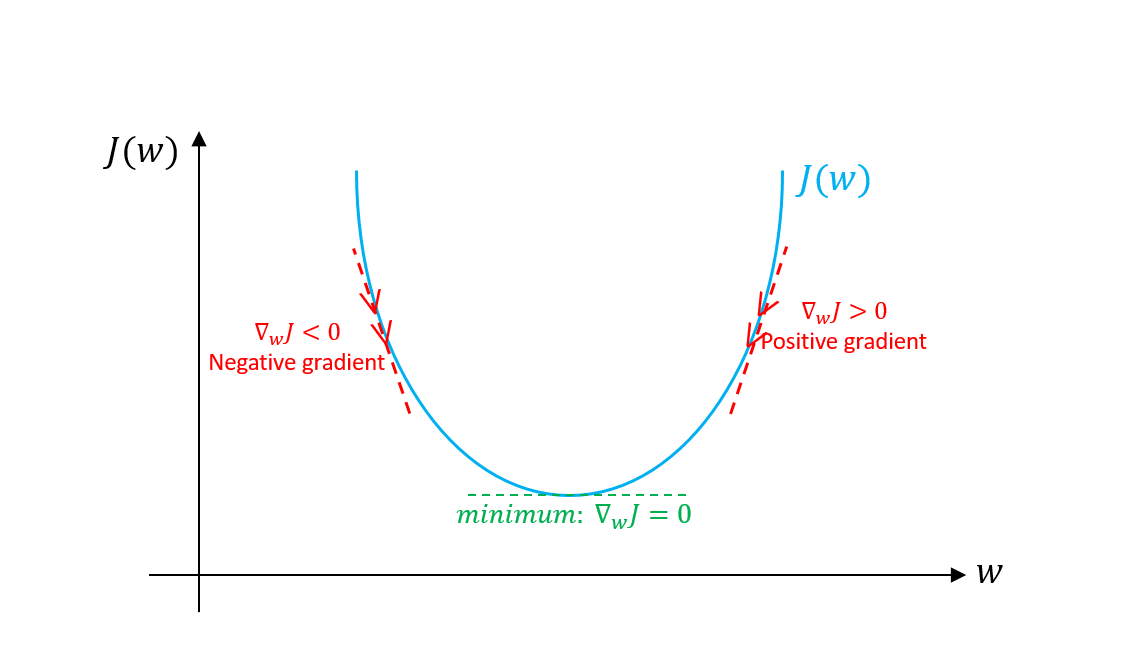
\includegraphics[width=0.8\columnwidth]{images/gradiente.png}
  \end{center}
  \caption{Vediamo come data una funzione, attraverso questo approccio si possa trovare il valore minimo.}
  \label{fig:Discesa del gradiente}
\end{figure}


\section{Deep Learning e Reti Neurali Artificiali}
Il Deep Learning è una branca del Machine Learning che mira ad estrarre delle rappresentazioni dei dati partendo dai dati stessi \cite{lecun2015deep}. La differenza sostanziale rispetto al Machine Lerning sta nel modo in cui vengono estratte le features: se nel Machine Learning occorreva la descrizione di un modello su cui basarsi per estrarle, con il Deep Learning non sarà più necessario. Le reti di Deep Learning infatti sono in grado di estrarre in modo del tutto autonomo queste features. Ovviamente per fare ciò occorre un enorme quantitativo di dati in più rispetto al Machine Learning ed è questo il motivo per il quale il Deep Learning si è sviluppato solo nell'ultimo periodo.

\begin{figure}[H]
  \begin{center}
    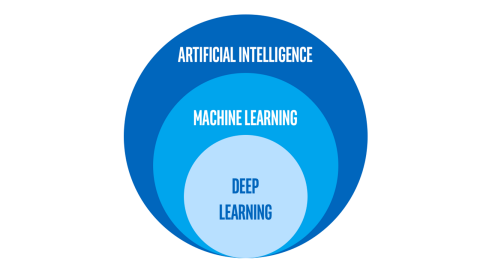
\includegraphics[width=0.8\columnwidth]{images/ai-machine-learning-deep-learning-rwd.png.rendition.intel.web.480.270.png}
  \end{center}
  \caption{Dalla figura capiamo come intelligenza artificiale, Machine Learning e Deep Learning siano strettamente connessi.}
  \label{fig:Artificial Intelligence Diagram}
\end{figure}

Le reti di Deep Learning sono costituite da strati detti \emph{layer}. In un algoritmo di Deep Learning ogni layer ha il compito di estrapolare una caratteristica specifica. Nelle elaborazioni delle immagini, ad esempio, i layer più bassi andranno a definire i bordi e le sfumature dell'immagine, mentre i layer più alti andranno invece a rilevare i concetti rilevanti per l'uomo, come la presenza di un viso o di una lettera.
Infine, per concludere questa panoramica iniziale sul Deep Learning occorre specificare cosa si intenda per \emph{hidden layer}, ovvero i layer nascosti. Gli hidden layer sono i layer interni alla nostra rete neurale, sono quei layer che mettono in comunicazione il primo layer, detto layer di input, con l'ultimo layer, detto layer di output, responsabile della produzione del risultato. Generalmente, per una rete neurale \emph{tradizionale} i layer nascosti sono 2-3, mentre per una rete neurale \emph{profonda}, tipica del Deep Learning, si arriva addirittura a 150 layer nascosti.
\\Vediamo ora come sono composti questi layer. Dicevamo come il compito di riconoscere un animale in foto fosse molto semplice da un punto di vista umano, mentre molto complesso per una macchina. L'ideale sarebbe avere una macchina dotata di \emph{cervello}, o comunque in grado di emulare il pensiero umano. E' proprio questa l'idea che è alla base delle reti neurali artificiali, ovvero le reti che vanno a comporre gli algoritmi di Deep Learning.
Le reti neurali umane sono un insieme di neuroni tra loro connessi, in grado di scambiare informazioni e di attivarsi o meno a seconda delle situazioni \cite{mehrotra1997elements}. Ricorda qualcosa? Esatto, è la funzione che hanno i layer in una rete di Deep Learning. Una rete neurale artificiale, è, quindi, un'emulazione delle reti neurali umane, composta da un grafo connesso di nodi, come si nota dalla figura \ref{fig:Artificial Neural Network}, all'interno del quale viaggiano le informazioni, o meglio i dati.

\begin{figure}[H]
  \begin{center}
    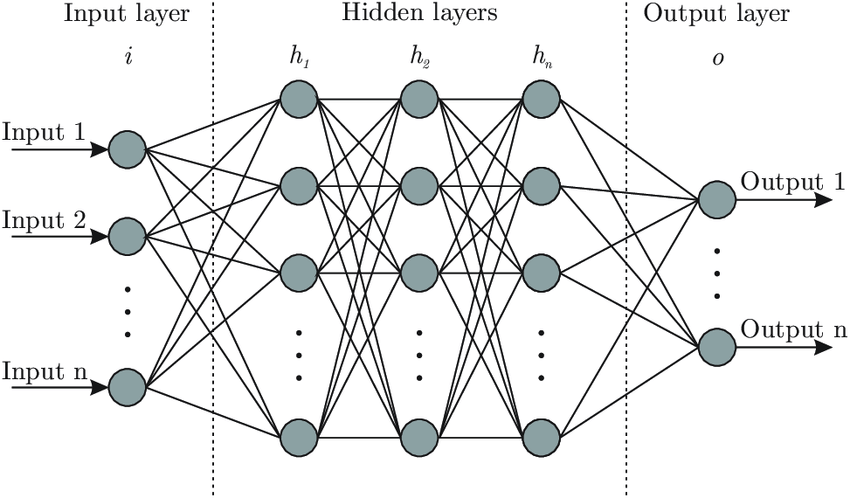
\includegraphics[width=0.8\columnwidth]{images/Artificial-neural-network-architecture-ANN-i-h-1-h-2-h-n-o.png}
  \end{center}
  \caption{Un esempio di rete neurale artificiale, notiamo la suddivisione in layer e come ogni neurone sia connesso ai neuroni del layer successivi}
  \label{fig:Artificial Neural Network}
\end{figure}

\section{Reti Neurali Convolutive}
Tra i tipi di reti neurali le rete neurali convolutive (CNN) sono le reti su cui fare riferimento quando si parla di visione artificiale ed elaborazione delle immagini \cite{yamashita2018convolutional}. Sono infatti reti in grado di catturare con successo ed efficienza le dipendenze spaziali e temporali delle immagini. Sono composte da tre blocchi o livelli: blocco convolutivo, blocco di pooling e i livelli completamente connessi. I primi due blocchi hanno il compito di estrarre le features, mentre il terzo ha il compito di mappare le features estratte nell'output finale. 
\\Per capire il loro funzionamento occorre analizzare come è definita un'immagine. Un'immagine non è altro come un insieme di pixel, ognuno con un determinato valore. Possiamo quindi vedere le immagini come una  matrice composta dai valori che assumono i pixel. Le immagini non sono però bidimensionali, infatti le immagini a colori sfruttano i tre canali RGB per comporre i colori, in questo caso avremo quindi una matrice con una dimensione tre di profondità, una per ogni canale. Per intenderci, un'immagine 4K avrà una definizione pari a 4096×2048, un numero quindi elevatissimo di pixel. E' proprio sulla dimensione che andremo a lavorare con il primo blocco delle rete neurali convolutive: vengono ridotte le dimensioni della matrice attraverso un'operazione di convoluzione, che dà il nome al blocco. Per descrivere il funzionamento definiamo il componente che ci permetterà di lavorare sulla matrice: il kernel, chiamato anche filtro. Il kernel può essere descritto come una matrice di pesi tipicamente di dimensione 3x3:
$$\begin{bmatrix}
w\textsubscript{11} & w\textsubscript{12} & w\textsubscript{13}\\
w\textsubscript{21} & w\textsubscript{22} & w\textsubscript{23}\\
w\textsubscript{31} & w\textsubscript{32} & w\textsubscript{33}
\end{bmatrix}$$
\\Il kernel ci permetterà di scorrere tutta l'immagine in altezza ed in larghezza, spostandoci ogni volta di una lunghezza definita a priori, e moltiplicare i valori con i pesi corrispondenti. Successivamente, questi valori verranno tra loro sommati ed andranno a comporre il nuovo valore della nuova matrice risultato, che avrà l'aspetto della figura \ref{fig:Kernel}.

\begin{figure}[H]
  \begin{center}
    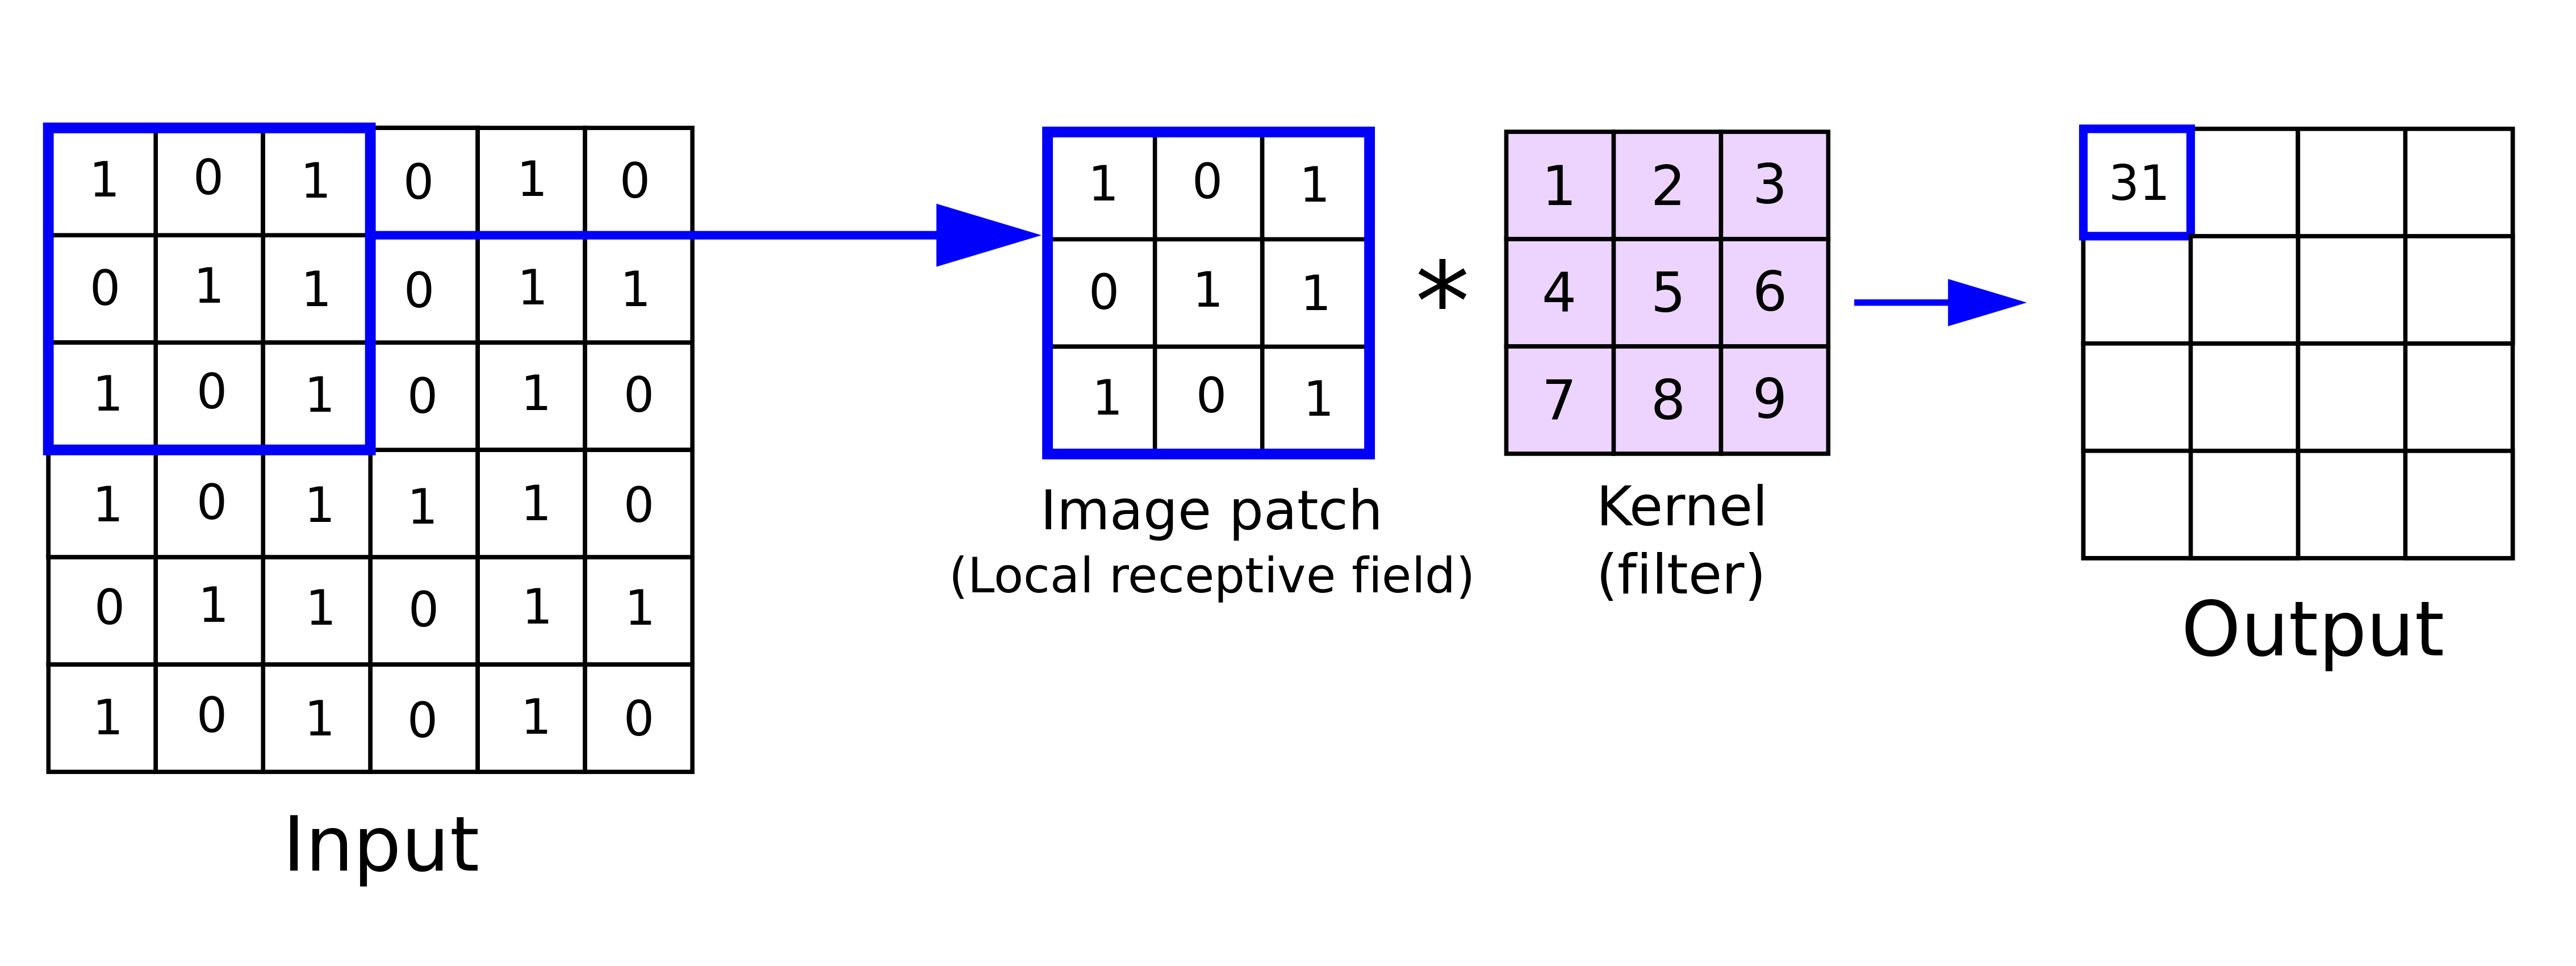
\includegraphics[width=0.8\columnwidth]{images/kernel.png}
  \end{center}
  \caption{Il kernel scorrerà tutta l'immagine al fine di creare una nuova matrice formata dalla somma dei valori dei pixel moltiplicati per i pesi.}
  \label{fig:Kernel}
\end{figure}
Quello che sta realmente accadendo è un'operazione di convoluzione sull'immagine al fine di rilevare caratteristiche come bordi, colore ed orientamento del gradiente.
Vi sono due tipi di approcci per questa operazione: il primo approccio, detto \emph{valid padding} permette di ottenere un risultato avente dimensione diversa rispetto alla matrice di partenza, mentre il secondo \emph{same padding} permette, aggiungendo ai margini della matrice iniziale colonne e righe composte da zeri, di ottenere una matrice avente la stessa dimensione di quella di partenza. Durante l'addestramento della rete, lo scopo sarà quello di trovare i valori dei pesi per i quali il kernel fornisce i risultati migliori. Dopo un'operazione di questo tipo, l'output viene fatto passare attraverso una funzione di attivazione, tipicamente una \emph{ReLu} che eliminerà i valori negativi.
\\Il secondo blocco, di pooling, avrà il compito di ridurre le dimensioni ulteriormente, al fine di ridurre la potenza di calcolo necessaria ad elaborare i dati, estrarrà le caratteristiche dominanti ed effettuerà una riduzione del rumore. Il compito di questo blocco sarà quello di ridurre le dimensioni della matrice e raggruppare i valori grazie all'utilizzo di un filtro unitario. Il filtro scorrerà tutta la matrice e, per ogni scorrimento, calcolerà un valore, che sarà il valore che andrà a comporre il risultato. Questo valore può essere calcolato secondo due approcci: \emph{max pooling} dove per ogni raggruppamento il risultato sarà il valore massimo, come in figura \ref{fig:Pooling}, oppure \emph{average pooling} dove per ogni raggruppamento il risultato sarà la media dei valori.
\begin{figure}[H]
  \begin{center}
    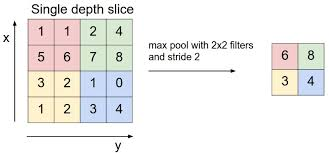
\includegraphics[width=0.8\columnwidth]{images/pooling.jpg}
  \end{center}
  \caption{In questo caso viene applicato l'approccio max pooling, vediamo come il filtro di dimensione 2x2 ricavi nel primo quadrante della matrice il valore massimo 6 e lo vada ad inserire nella matrice risultato.}
  \label{fig:Pooling}
\end{figure}
Abbiamo visto quindi come vengano catturate le caratteristiche principali della nostra immagine grazie ai primi due blocchi della rete, ora il compito passerà all'ultimo blocco il quale avrà il compito di convertire i risultati fin'ora ottenuti nella forma adatta agli output finali della rete.
\\Le CNN sono molteplici, successivamente ci concentreremo sull'architettura ResNet che descrive la rete del nostro progetto.


\section{Generative Adversarial Network}
Le Generative Adversarial Netwrok (GAN) sono un modello generativo basato sul Deep Learning \cite{brownlee2019generative} utilizzato per la creazione di immagini. Si tratta di un modello basato su due reti: una rete discriminativa, che ha lo scopo di determinare se un'immagine è reale, oppure falsa, ed una rete generativa, il quale compito è appunto quello di generare immagini. Per capire meglio il loro funzionamento aiutiamoci con un paragone: la rete discriminatrice possiamo vederla come un poliziotto, mentre la rete generatrice come un contraffattore. Lo scopo del contraffattore è quello di affinare la propria abilità al fine di produrre opere false e riuscire a spacciarle per vere senza farsi scoprire, mentre lo scopo del poliziotto è quello di ostacolare il contraffattore rilevando se un'opera è reale o meno. La competizione generata da questo duello porta entrambi a migliorarsi, fino a quando non si arriverà al punto in cui il contraffattore riesce a riprodurre opere indistinguibili da quelle reali \cite{goodfellow2014generative}.
\\
Andiamo ora a descrivere queste reti e la teoria sulla quale si basano.
\\Prima di tutto occorre parlare di una tipologia differente da quella fin'ora trattata di addestramento: l'addestramento non supervisionato. Abbiamo visto come durante la fase di addestramento gli esempi forniti alla rete vengano associati ad un valore di uscita $y$ e di come la rete si addestri su questi valori. Nell'addestramento non supervisionato, a differenza, agli esempi di addestramento, non vengono associate le uscite $y$, ma vengono forniti solo gli input. L'obiettivo di questo addestramento è quello di rendere la rete in grado di rilevare una correlazione tra gli esempi e, di conseguenza, di ricavare un modello. E' ciò che sta alla base dei modelli generativi, ovvero i modelli in grado di generare nuovi elementi il quanto più possibile simili agli elementi dell'insieme di input.
\\
Dicevamo di come il modello fosse suddiviso in Generatore e Discriminatore, andiamo ora a vedere come lavorano.
\\Partendo inizialmente da un vettore casuale $z$, il generatore $G$ genererà un'immagine fake $G(z)$. Questa immagine sarà poi data in ingresso al Discriminatore $D$, che dovrà determinare se l'immagine è reale o falsa, dovrà quindi fare una predizione $D(G(z))$. Sul risultato di questa previsione verrà calcolata la funzione d'errore del discriminatore e, con il metodo già ampiamente descritto della discesa del gradiente, verrà addestrato, mantentenendo invariati i parametri del Generatore. Sempre con lo stesso metodo verrà successivamente addestrato il Generatore.
\\Le funzioni d'errore utilizzate nell'addestramento di queste reti sono logaritmiche. Supponiamo il caso di un'immagine reale, i casi possono essere due:
\begin{itemize}
    \item la previsione è conforme all'immagine, ovvero, determinato con 1 il valore dell'immagine reale, la previsione sarà un valore ad esso vicino, ad esempio $D(x)=0.9$, per cui l'errore commesso sarà piccolo
    \item la previsione è errata, ad esempio $D(x)=0.1$, per cui l'errore commesso sarà grande
\end{itemize}
Una funzione che si comporta come quanto descritto è $f=-log(D(x))$, che nel nostro caso avrà come risultato: $f=0.1$ per $D(x)=0.9$ e $f=2.3$ per $D(x)=0.1$. Come visto questa funzione approssima bene il comportamento che vogliamo ottenere dalla funzione d'errore, ovverò è elevata tanto più la previsione è errata.
\\Con calcoli analoghi, si ottiene come risultato $f=-log(1-D(G(z))$ nel caso in cui l'immagine sia generata dal Generatore. Quindi, dato che l'obiettivo della rete è quello di generare un'immagine finta indistinguibile da una reale, l'apprendimento consisterà quindi nell'ottimizzare un gioco \emph{minmax} per $G$ e $D$:
$$
{\displaystyle \min _{G}\max _{D}\mathbb {E} _{{\boldsymbol {x}}\sim p_{data}({\boldsymbol {x}})}[\log D({\boldsymbol {x}})]+\mathbb {E} _{{\boldsymbol {z}}\sim p_{\boldsymbol {z}}({\boldsymbol {z}})}[\log(1-D(G({\boldsymbol {z}})))]}
$$
\\L'utilizzo delle GAN si concentra su tre campi principali:
\begin{itemize}
    \item Image Super-Resolution, per migliorare la qualità delle immagini in ingresso;
    \item Creare arte;
    \item Image to Image Translation, ovvero l'applicazione di uno stile ad un'immagine di input, come ad esempio estate-inverno, giorno-notte, e, come vedremo più avanti nel nostro caso, cavallo-zebra. Un esempio di questa applicazione è mostrato in figura \ref{fig:HorsetoZebra Example}.
\end{itemize}

\begin{figure}[H]
  \begin{center}
    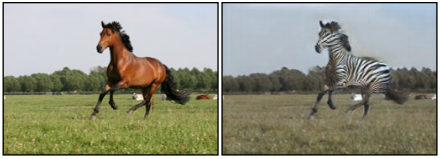
\includegraphics[width=0.8\columnwidth]{images/cyclegan example.png}
  \end{center}
  \caption{Un esempio di Image to Image translation  \cite{Zhu_2017_ICCV}}
  \label{fig:HorsetoZebra Example}
\end{figure}
\subsection{Pix2Pix Translation}
Un aspetto da sottolineare per quanto riguarda le GAN è la possibilità di condizionarne il funzionamento. Parliamo quindi di Conditional Generative Adversarial Network, utilizzate nella traduzione da immagine a immagine Pix2Pix \cite{goodfellow2014generative}.
\\Abbiamo visto come le GAN generino delle immagini partendo dal rumore. L'idea che è alla base di questa traduzione è quella di partire a generare un'immagine non più da un vettore casuale ottenuto dal rumore, bensì da un'altra immagine \cite{isola2018imagetoimage}. Aiutandoci con un esempio, supponiamo di avere una GAN utilizzata nella generazione di visi umani. Dalla GAN in questione ci aspettiamo che la probabilità di generare un volto femminile sia pari a quella di un volto maschile, e che quindi la rete non faccia distinzione sull'output generato. Utilizzando una GAN condizionata possiamo, appunto, condizionare la generazione dei volti solo su quelli femminili o solo su quelli maschili. Per fare ciò addestreremo la rete non più su una singola immagine come visto fin'ora, ma su coppie di immagini, grazie ad un dataset \emph{paired}, ovvero un dataset composto da immagini accoppiate a due a due secondo la relazione input-output \cite{Zhu_2017_ICCV}. In questo modo il discriminatore non lavorerà più facendo previsioni solamente sull'immagine generata, ma lo farà sulla coppia di immagini: immagine di partenza più immagine generata e immagine di partenza più rispettivo output, come si nota dall'esempio in figura \ref{fig:Pix2Pix}.


 \begin{figure}[H]
  \begin{center}
    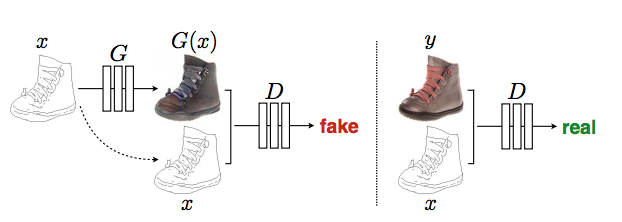
\includegraphics[width=0.8\columnwidth]{images/pix2pix.png}
  \end{center}
  \caption{Vediamo come il discriminatore esegua una previsione sulla coppia di immagini input-output fake e input-output associato.}
  \label{fig:Pix2Pix}
\end{figure}


\section{GradCam}
Abbiamo ampiamente parlato di CNN e di come il loro funzionamento sia ideale o molto performante nell'ambito della visione artificiale e dell'elaborazione delle immagini. Come per ogni ambito dell'intelligenza artificiale, è molto importante capire il loro funzionamento e renderle il più intuitive possibili. Questo perchè, nel caso di un malfunzionamento, occorre sapere da che cosa è stato determinato. La necessità di comprendere in maniera trasparente il loro funzionamento è data da tre principali motivi. In primo luogo, quando l'AI è debole rispetto alla capacità umana è utile identificare il perchè il suo comportamento fallisca. Successivamente quando l'AI è pari alla capacità umana l'obiettivo è quello di stabilire un'adeguata fiducia negli utenti. Infine, quando l'AI è decisamente superiore all'intelligenza umana l'obiettivo è quello di apprendere da essa \cite{Selvaraju_2017_ICCV}.
\\Una delle tecniche principali per capire il funzionamento delle CNN è attraverso le mappe di attivazione di classe (CAM). La loro logica è basata sui risultati che produce l'ultimo livello convolutivo di una CNN. Sostanzialmente, grazie alle features map prodotte dall'ultimo layer convolutivo è possibile ricavare dove si focalizza l'attenzione della rete. Per rendere più chiaro il concetto riprendiamo l'esempio della rete classificatrice. Vogliamo capire dove si concentra la rete, su che parametri dell'immagine. Ci aspettiamo che difficilmente l'attenzione sia focalizzata ai margini dell'immagine, o su parametri secondari come lo sfondo, ma che sia focalizzata sulla sagoma dell'animale. CAM ci permette, grazie ad una mappa del calore come vediamo in figura \ref{fig:GradCam example}, di verificare come si comporti la rete nell'analisi dell'immagine.

\begin{figure}[H]
  \begin{center}
    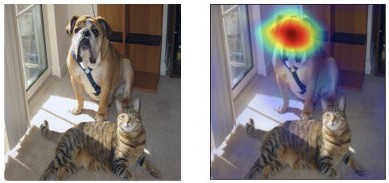
\includegraphics[width=0.8\columnwidth]{images/gradcam example.jpg}
  \end{center}
  \caption{Il risultato dell'applicazione di GradCam su una rete classificatrice. In questo caso l'output di classificazione riguarda il cane e vediamo come l'attenzione sia concentrata tutta sulla faccia dell'animale.}
  \label{fig:GradCam example}
\end{figure}
L'approccio visto fin'ora funziona però solo su reti CNN e non su altre architetture. Introduciamo quindi GradCam, avente un funzionamento simile a quanto descritto, ma applicabile a qualsiasi tipologia di architettura.
Vediamone il funzionamento nel dettaglio. Sia la nostra rete una rete classificatrice e sia $y\textsuperscript{c}$ l'output di classificazione della rete. Denotiamo inoltre con $A\textsuperscript{k}$ le mappe di attenzione generate dall'ultimo layer convolutivo della rete sulle quali vogliamo andare a calcolare l'attenzione. Calcoliamo il gradiente di $y\textsuperscript{c}$ rispetto alle mappe di attenzione $A\textsuperscript{k}$:
$$\frac{\partial y\textsuperscript{c}}{\partial A\textsuperscript{k}}
$$
Ora, applichiamo un \emph{global average pooling}, ovvero la media su altezza e larghezza di ogni mappa di attenzione, e poniamo:
$$\alpha\textsuperscript{c}\textsubscript{k} =
\frac{1}{Z} \sum_{i=1} \sum_{j=1} \frac{\partial y\textsuperscript{c}}{\partial A\textsuperscript{k}\textsubscript{ij}}$$
$\alpha\textsuperscript{c}\textsubscript{k}$ sarà un vettore di dimensione pari al numero di feature map del layer scelto e conterrà i pesi da affidare ad ogni feature map.
\\Successivamente moltiplicheremo il vettore contenente i pesi con le features map e ne faccremo una somma. In questo modo associamo ad ogni canale della convoluzione un peso determinato dal gradiente. Il peso associato a questi canali indica se si attivano o meno durante l'elaborazione dell'immagine. Infine applicheremo una ReLu alla somma ottenuta, al fine di eliminare i valori negativi. \\Il risultato ottenuto potrà essere visto attraverso una mappa del calore ed indicherà dove sarà maggiormente focalizzata l'attenzione della rete nel layer stabilito.

\section{Fréchet Inception Distance}
Definite le GAN, definito GradCam come metodo per visualizzare dove le reti vanno a lavorare, occorre ora definire un metodo per valutare la qualità della rete generatrice. Introduciamo quindi il Fréchet Inception Distance (FID). Il FID è un metodo utilizzano per valutare la qualità delle immagini generate da una GAN \cite{DBLP:journals/corr/HeuselRUNKH17}. Il metodo si basa sul concetto matematico della distanza di Fréchet utilizzato in matematica per calcolare la somiglianza tra le curve tenendo conto della posizione e dell'ordine dei punti lungo le curve \cite{eiter1994computing}. Il ragionamento è quello di valutare due insiemi: un insieme di esempio e un insieme di immagini generate dalla rete. Vengono calcolate quindi le distribuzioni di questi due insiemi, vengono confrontate e viene prodotto un risultato. Il risultato indicherà quanto sono distanti le due distribuzioni, quindi un risultato piccolo è ottimale. 

         \chapter{Sistema Realizzato}
In questo capitolo illustreremo l'architettura del nostro progetto e andremo ad analizzare il codice. Partiremo con la definizione del problema della traduzione da immagine a immagine e vedremo com'è composta la rete che abbiamo utilizzato.

\section{Image to Image Translation}
(Ho pensato di strutturarla così: breve introduzione sul problema, spiegazione sul perchè pix2pix non sia la soluzione che usiamo, introduzione a cyclegan)\\
Vi siete mai chiesti come sarebbe bello poter ottenere una foto a colori da una foto in bianco e nero? Oppure avere la possibilità di passare da una foto ritraente un paesaggio estivo a un paesaggio autunnale?
\\Questi sono solamente alcuni degli esempi di applicazioni della image-to-image translation. L'image-to-image translation è molto simile a ciò che accade nella traduzione da lingua a lingua: partendo da un'immagine appartenente ad un dominio iniziale, come la foto di un paesaggio estivo, vogliamo ottenere un'immagine appartenente ad un altro dominio, ad esempio passando da paesaggio estivo a paesaggio autunnale.
\\Un esempio di image-to-image translation è il già trattato Pix2Pix \cite{isola2018imagetoimage} che, grazie ad una GAN condizionata addestrata con un training set \emph{paired}, di cui un esempio in figura \ref{fig:Paired and Unpaired training set}, produce un output condizionato dall'immagine di input.
\\Tuttavia, l'approccio Pix2Pix fin qui descritto non è del tutto efficiente in quanto il training set della rete comporta un notevole sforzo nella sua creazione. Infatti, tornando all'esempio dei paesaggi, occorrebbe avere un enorme quantitativo di foto ritraenti lo stesso identico paesaggio in due differenti momenti dell'anno. In aggiunta, per alcune applicazioni sarebbe del tutto impossibile ottenere un training set di questo tipo: basti pensare alla traduzione da opere d'arte a foto, o all'applicazione di uno stile a immagini reali, come vedremo più avanti nel nostro caso quando vorremo trasformare cavalli in zebre e viceversa.

\begin{figure}[H]
  \begin{center}
    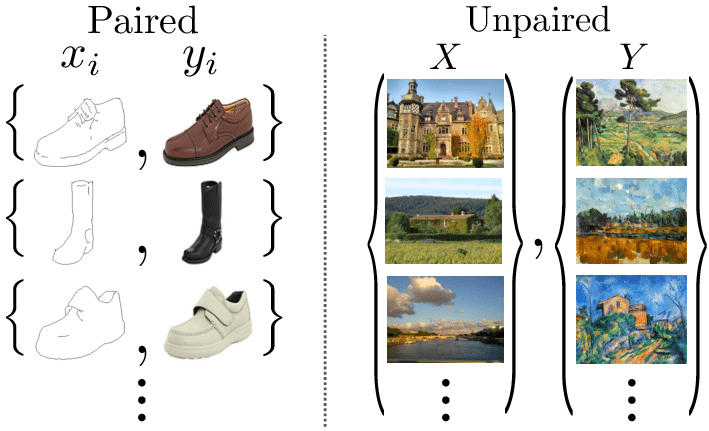
\includegraphics[width=0.8\columnwidth]{images/Paired-training-data-left-consists-of-training-examples-x-i-y-i-N-i1-where-the.png}
  \end{center}
  \caption{Vediamo un esempio di set paired, dove le immagini sono accoppiate tra input-outpu e set unpaired dove non vi è questa corrispondenza.}
  \label{fig:Paired and Unpaired training set}
\end{figure}
Proprio per questo motivo si è pensato di adottare una nuova soluzione attraverso l'addestramento con un training set \emph{unpaired}, dove non vi è una corrispondenza di input-output accoppiati, come vediamo sempre in figura \ref{fig:Paired and Unpaired training set}. In questo caso l'obiettivo è quello di addestrare una rete in grado di mappare le immagini appartenenti al dominio di partenza nel dominio di arrivo, in modo tale che le immagini generate siano verosimilmente appartenenti al dominio di arrivo.
\\Tuttavia non siamo ancora arrivati ad un risultato ottimale che soddisfi le nostre esigenze per la traduzione di un'immagine: in questo modo, infatti, non stiamo garantendo la traduzione esatta da immagine di input a immagine di output, ne stiamo solo condizionando la creazione. Inoltre potrebbe subentrare il problema del collasso della rete, dove tutte le immagini di input si mappano nella stessa immagine di output \cite{Zhu_2017_ICCV}.
Occorre quindi trovare un modo per migliorare l'idea fin qui realizzata, e proprio per questo motivo introduciamo una nuova architettura: la Cycle GAN.

\section{Cycle GAN}
(Ho pensato di strutturarla così: introduzione, spiegazione matematica del funzionamento della consistenza del ciclo, implementazione per la classe networks.py e cycle-gan-model.py (solo le funzioni importanti), addestramento)\\
Per spiegare questa architettura possiamo fare un paragone con la linguistica. Quando vogliamo tradurre una frase dall'italiano all'inglese vogliamo che applicando il procedimento di traduzione inversa da inglese a italiano, la frase torni ad essere quella di partenza. Vogliamo cioè che vi sia della consistenza tra i risultati. Questo concetto è ciò proprio che vogliamo applicare al nostro problema della traduzione da immagine a immagine. In poche parole vogliamo ottenere un'immagine di output, la quale applicando a ritroso la traduzione ci restituisca come risultato l'immagine di input. 
\\Matematicamente non vogliamo far altro che trovare due funzioni biettive $G:X\rightarrow{}Y$ e $F:Y\rightarrow{}X$, tali per cui $F$ sia l'inversa di $G$, ovvero:
$$\begin{cases}
  F(G(x))=x\\
  G(F(y))=y  
\end{cases}
$$
Da un punto di vista architetturale questo problema può essere risolto attraverso due reti GAN, la prima responsabile della traduzione da $X$ a $Y$, la seconda resposabile della traduzione inversa da $Y$ a $X$ \cite{Zhu_2017_ICCV}. In questo modo il generatore della prima rete prenderà in input le immagini dal primo dominio e produrrà in output le immagini per il secondo dominio, successivamente il compito passerà al generatore della seconda rete che prenderà come input le immagini generate dal primo generatore e produrrà come output un'immagine del primo dominio il più fedele possibile, poi vedremo come, all'immagine di partenza. I rispettivi discriminatori saranno impiegati nel determinare quanto le immagini generate siano plausibili. 
\\Per quanto riguarda l'addestramento, esso è conforme a quanto già descritto per le reti GAN, con l'aggiunta di una loss che indica la consistenza del ciclo. Per spiegare come viene calcolata questa loss aggiuntiva definiamo due concetti: \emph{forward cycle consistency} e \emph{backward cycle consistency}. Il forward cycle consistency (consistenza del ciclo in avanti) non è altro che la sopra definita $F(G(x))=x$, mentre il backward cycle consistency (consistenza del ciclo all'indietro) è la sopra definita $G(F(Y))=y$, come si può intuire visivamente dalla figura \ref{fig:Cycle Consistency}. Attraverso questi due concetti possiamo quindi valutare di quanto si discosta l'immagine rigenerata, grazie al forward cycle consistency, con l'immagine iniziale. Infatti, calcolando la differenza (che matematicamente rappresentiamo con la norma, o la norma al quadrato) tra le due immagini si ottiene l'errore che la rete commette durante la traduzione dell'immagine. Possiamo applicare il medesimo ragionamento per quanto riguarda il backward cycle consistency per ottenere la loss di consistenza del ciclo:
$$L\textsubscript{cyc}(G,F) = ||G(F(x))-x|| + ||F(G(Y))-y||$$

\begin{figure}[H]
  \begin{center}
    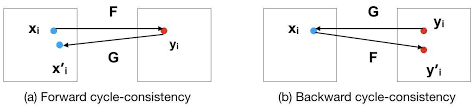
\includegraphics[width=0.8\columnwidth]{images/cycle consistency.png}
  \end{center}
  \caption{Vediamo una rappresentazione grafica della consistenza del ciclo.}
  \label{fig:Cycle Consistency}
\end{figure}
In questo modo abbiamo quindi definito una rete costituita da due GAN cicliche, da cui il nome. La loss totale della rete dipenderà quindi dalle loss delle due GAN, più la loss aggiuntiva che indica la consistenza del ciclo.
$$L\textsubscript{cycgan}(G,F,D\textsubscript{x},D\textsubscript{y})=
L\textsubscript{gan}(G,D\textsubscript{y},X,Y) +
L\textsubscript{gan}(F,D\textsubscript{x},Y,X) + 
L\textsubscript{cyc}(G,F)
$$
Come ampiamente spiegato la Cycle GAN può essere definita attraverso due funzioni biettive, una l'inversa dell'altra. Un problema di traduzione da immagine a immagine risolto attraverso l'implementazione di una rete di questo tipo porterà quindi ad una doppia soluzione: la traduzione, che possiamo definire \emph{primaria}, da dominio $A$ a dominio $B$ ed una traduzione \emph{secondaria} da dominio $B$ a dominio $A$.
Vedremo infatti nei capitoli futuri come il nostro progetto si concentri sulla traduzione di immagini da cavalli a zebre, ma noteremo come, seppur con risultati inferiori, la rete sia in grado di tradurre anche da zebre a cavalli, come vediamo tra gli esempi di figura \ref{fig:Cycle GAN Example}.

\begin{figure}[H]
  \begin{center}
    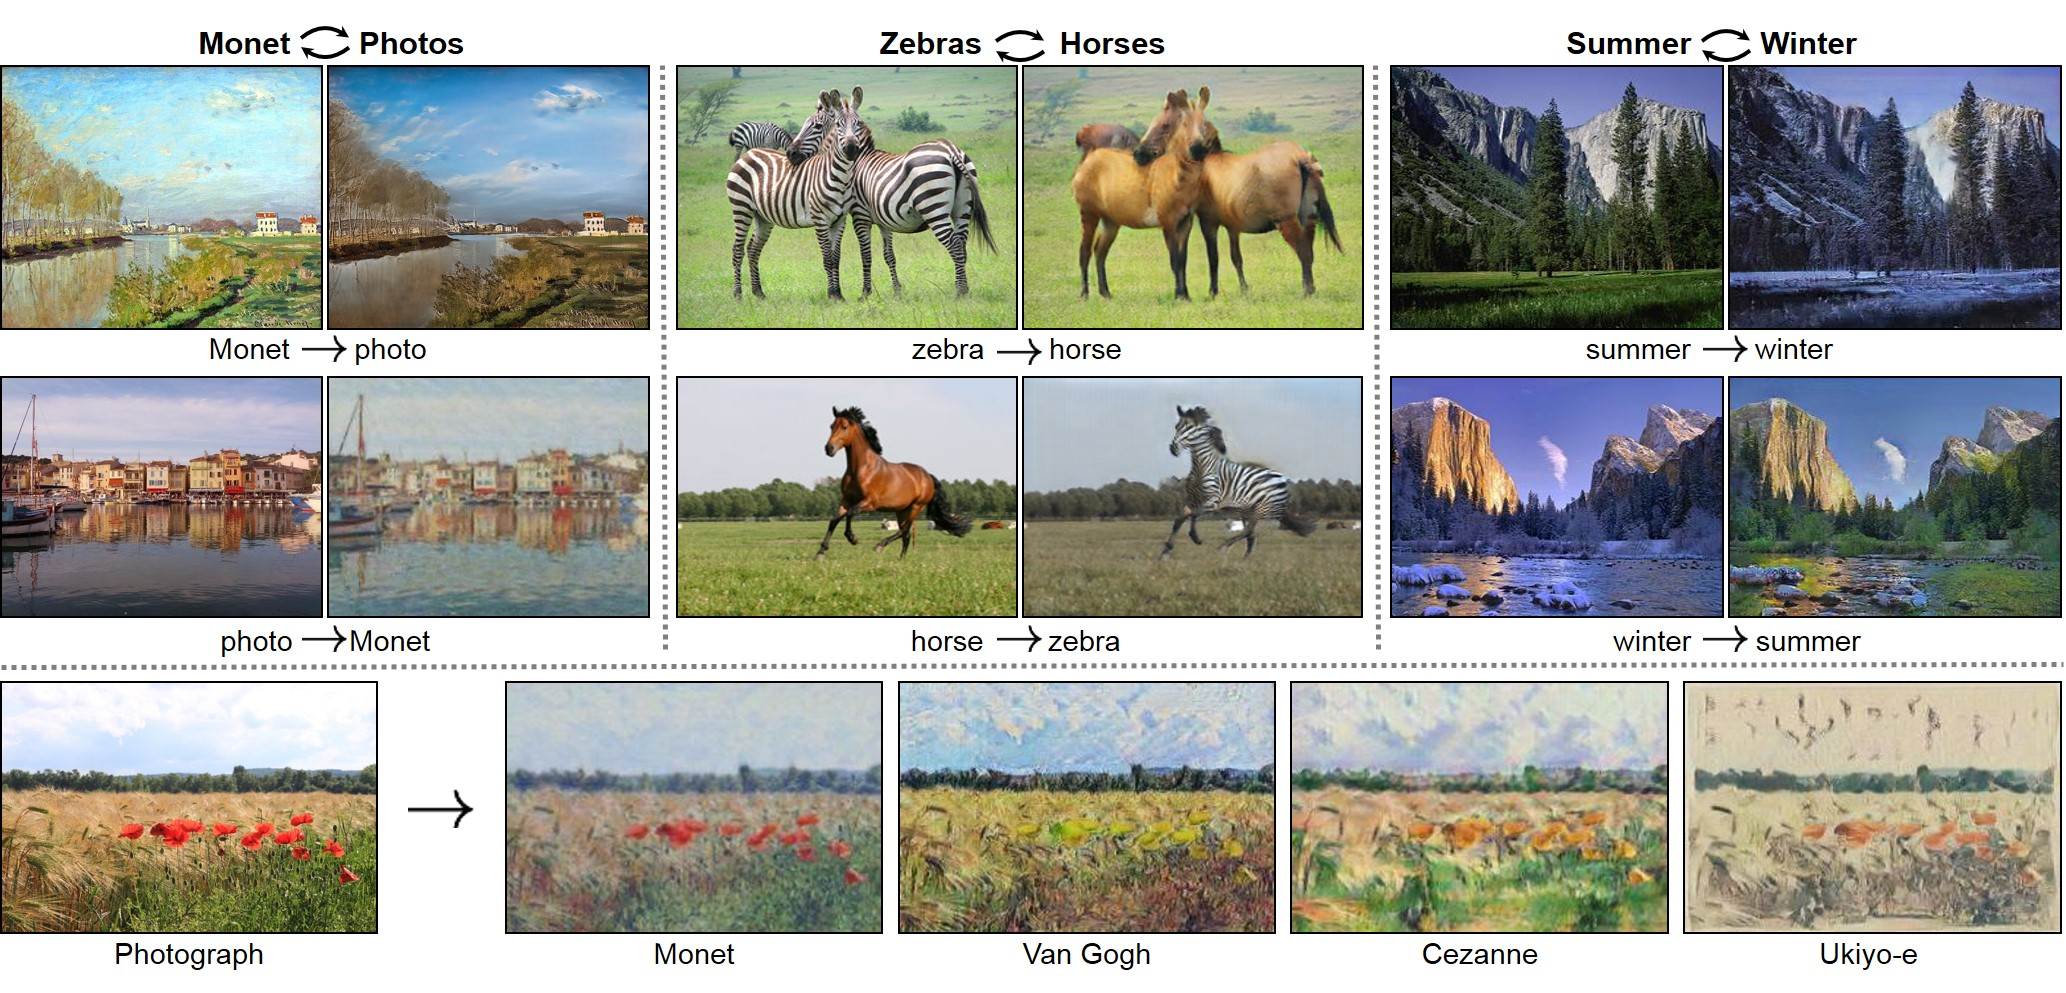
\includegraphics[width=1\columnwidth]{images/cycle gan example.jpg}
  \end{center}
  \caption{Vediamo vari esempi di una image to image translation attraverso l'uso di Cycle GAN.}
  \label{fig:Cycle GAN Example}
\end{figure}

\section{Codice ed Implementazione}
Dopo aver trattato la teoria sulla quale si basano le Cycle GAN vediamo in questa sezione com'è possibile implementarle a livello di codice. L'implementazione iniziale da cui partiremo è quella proposta dal  \href{https://github.com/junyanz/pytorch-CycleGAN-and-pix2pix}{Paper} \cite{Zhu_2017_ICCV}.
\\Il codice è scritto in Python e utilizza il Framework Pytorch per costruire la rete e addestrarla. Il codice dà la possibilità di specificare diversi parametri utili alla rete, in questa sezione ci limiteremo a definire quelli utilizzati nel nostro progetto.
\subsection{Networks}
La prima classe che andiamo a definire è la classe \href{https://github.com/junyanz/pytorch-CycleGAN-and-pix2pix/blob/master/models/networks.py}{networks}, all'interno della quale vengono definite le architetture utilizzate per implementare la CycleGAN.
Come prima cosa andremo a definire le reti Generatrici, che nel nostro progetto saranno composte attraverso un'architettura ResNet avente nove blocchi residui. Notiamo come durante l'inizializzazione del Generatore sia possibile andare a specificare alcuni parametri, per cambiare il comportamento della rete. Tra questi troviamo la tipologia dell'architettura utilizzata, la quale, nel nostro caso, sarà, come detto, una ResNet.

\begin{minted}[bgcolor=lightGray]{python}
ResnetGenerator(
    (model): Sequential(
      (0): ReflectionPad2d
      (1): Conv2d
      (2): InstanceNorm2d
      (3): ReLU
      (4): Conv2d
      (5): InstanceNorm2d
      (6): ReLU
      (7): Conv2d
      (8): InstanceNorm2d
      (9): ReLU
      (10): ResnetBlock
      (11): ResnetBlock
      (12): ResnetBlock
      (13): ResnetBlock
      (14): ResnetBlock
      (15): ResnetBlock
      (16): ResnetBlock
      (17): ResnetBlock
      (18): ResnetBlock
      (19): ConvTranspose2d
      (20): InstanceNorm2d)
      (21): ReLU
      (22): ConvTranspose2d
      (23): InstanceNorm2d
      (24): ReLU
      (25): ReflectionPad2d
      (26): Conv2d
      (27): Tanh
    )
)

\end{minted}
Con codice analogo vengono successivamente definite le reti Discriminatrici. Anche in questo caso sarebbe possibile specificare ulteriori parametri per cambiare il tipo di rete utilizzato. Si distinguono tre tipologie di Discriminatore: \emph{basic}, \emph{n-layer} e \emph{pixel}. Nella nostra rete utilizzeremo il discriminatore Basic, il quale suddivide l'immagine in parti composte da 70x70 pixel e per ognuna di queste viene effettuata una classificazione tra reale e fake.
\begin{minted}[bgcolor=lightGray]{Python}
NLayerDiscriminator(
    (model): Sequential(
      (0): Conv2d
      (1): LeakyReLU
      (2): Conv2d
      (3): InstanceNorm2d
      (4): LeakyReLU
      (5): Conv2d
      (6): InstanceNorm2d
      (7): LeakyReLU
      (8): Conv2d
      (9): InstanceNorm2d
      (10): LeakyReLU
      (11): Conv2d
    )
  )
\end{minted}


Successivamente viene definita la Loss della GAN, nel nostro progetto utilizzeremo una \emph{Mean Squared Error Loss}:
$${\displaystyle MSE={\frac {\sum _{i=1}^{n}(x_{i}-{\widehat {x}}_{i})^{2}}{n}}}$$
Proseguendo all'interno del codice vengono definiti i blocchi residui della nostra ResNet. Come detto in precedenza la nostra rete sarà composta da nove blocchi residui. I blocchi residui vengono utilizzati nel Deep Learning al fine di poter ottenere una maggiore profondità della rete. Infatti, se anzichè utilizzare una ResNet utilizzassimo un'altra architettura, sarebbe errato parlare di precisione della rete proporzionale alla sua profondità, in quanto subentrerebbe il problema del \emph{vanishing gradient}, secondo il quale il gradiente si annullerà a causa dei troppi livelli. Per questo motivo vengono introdotte le ResNet, le quali attraverso \emph{salti} tra i layer che compongono i blocchi residui, riescono ad evitare questo problema \cite{targ2016resnet}.
\\Ogni blocco residuo è composto da i seguenti layer:
\begin{minted}[bgcolor=lightGray]{Python}
ResnetBlock(
    (conv_block): Sequential(
      (0): ReflectionPad2d
      (1): Conv2d
      (2): InstanceNorm2d
      (3): ReLU
      (4): ReflectionPad2d
      (5): Conv2d
      (6): InstanceNorm2d
    )
\end{minted}
\subsection{Cycle GAN Model}
Dopo aver descritto come viene definita l'architettura della rete, possiamo descrivere come la Cycle GAN è implementata. 
\\Come prima cosa occorre ovviamente costruire i due generatori e i due discriminatori, richiamando i sopra citati metodi della classe networks.
Successivamente definiamo il comportamento dei Generatori che avranno il compito di generare le immagini fake attraverso le quali andremo a calcolare la Loss:
\begin{minted}[bgcolor=lightGray]{Python}
def forward(self):
    self.fake_B = self.netG_A(self.real_A)  # G_A(A)
    self.rec_A = self.netG_B(self.fake_B)   # G_B(G_A(A))
    self.fake_A = self.netG_B(self.real_B)  # G_B(B)
    self.rec_B = self.netG_A(self.fake_A)   # G_A(G_B(B))
\end{minted}
Come vediamo le istruzioni rappresentano il funzionamento descritto per le Cycle GAN: partendo da un'immagine del dominio $A$, generiamo con il primo generatore un'immagine fake per il dominio $B$, successivamente attraverso il secondo generatore ricostruiamo l'immagine iniziale partendo dall'immagine fake del dominio $B$. Questo procedimento è ripetuto in maniera analoga anche per la generazione da dominio $B$ a dominio $A$.
\\Seguentemente definiamo la funzione Backward per i due discriminatori, alla quale passiamo come argomenti le immagini reali e le immagini fake, su cui i discriminatori dovranno effettuare la previsione, al fine di calcolare la Loss dei discriminatori.
\begin{minted}[bgcolor=lightGray]{Python}
def backward_D_basic(self, netD, real, fake):
    pred_real = netD(real)
    loss_D_real = self.criterionGAN(pred_real, True)
    # Fake
    pred_fake = netD(fake.detach())
    loss_D_fake = self.criterionGAN(pred_fake, False)
    # Combined loss and calculate gradients
    loss_D = (loss_D_real + loss_D_fake) * 0.5
    loss_D.backward()
\end{minted}
Infine definiamo il metodo di Backward per quanto riguarda i generatori: è qui che calcoleremo la Loss di consistenza del ciclo. 
\begin{minted}{Python}
# Forward cycle loss || G_B(G_A(A)) - A||
self.loss_cycle_A = self.criterionCycle(self.rec_A, self.real_A)
# Backward cycle loss || G_A(G_B(B)) - B||
self.loss_cycle_B = self.criterionCycle(self.rec_B, self.real_B)
\end{minted}
Oltre alla Loss di consistenza del ciclo sono ovviamente presenti le classiche Loss per le reti GAN e una Loss di identità ottenuta passando ad un generatore un'immagine del dominio di arrivo, teoricamente il generatore in questione dovrebbe produrre come output l'immagine stessa in quanto già appartenente al dominio d'arrivo.

\section{Addestramento}
Abbiamo quindi definito tutti i punti più importanti delle classi che definiscono la nostra rete, ora possiamo concentrarci sull'addestramento. Per prima cosa occorre definire un dataset sul quale andare a lavorare. Il progetto dal quale siamo partiti mette a disposizione svariati dataset su cui addestrare la rete, tra questi il dataset \emph{horse2zebra}. Il dataset in questione offre la possibilità di tradurre immagini di cavalli in zebre, quindi applicando le strisce bianche e nere al manto del cavallo, e da zebre a cavalli, quindi applicando il procedimento inverso rimuovendo le strisce bianche e nere e dando un colore omogeneo al manto.
\\Per l'addestramento della rete si è scelto di utilizzare Google Colab, un ambiente gratuito offerto dalla Google che mette a disposizione le proprie schede grafiche per addestrare reti di questo tipo. 
\\L'addestramento si basa su epoche e per la nostra rete il numero di epoche fissato è pari a 200.
\\Per quanto riguarda i tempi di addestramento essi ovviamente variano a seconda della rete che si vuole addestrare. Nel nostro caso i tempi impiegati dalla Cycle GAN fin qui descritta erano dell'ordine dei minuti per epoca, indicativamente dieci. Per le modifiche successive che apporteremo alla rete vedremo come il tempo necessario all'addestramento aumenterà, fino ad arrivare a oltre quaranta minuti per epoca per la Cycle GAN addestrata grazie all'utilizzo di GradCam su quattro blocchi residui, che descriveremo nei capitoli successivi.


\section{GradCam}
(Ho pensato di strutturarla così: richiamo a quanto fa gradcam definito nei capitoli precedenti, spiegazione del perchè utilizziamo gradcam, definizione parametri usati (layer e output classificazione), spiegazione codice, implementazione gradcam e cyclegan)\\
Nel capitolo precedente abbiamo trattato l'algoritmo GradCam definendolo come un algoritmo in grado di associare una risposta visiva al comportamento della rete, indicandoci attraverso una mappa di calore dove la rete pone la propria attenzione durante la generazione delle immagini. L'idea è quindi quella di sfruttare GradCam al fine di indirizzare l'attenzione della rete durante la generazione delle immagini. Idealmente, infatti, le mappe di attenzione durante la ricostruzione dell'immagine iniziale, quindi dal dominio $B$ al dominio $A$, dovrebbero essere uguali a quelle della trasformazione da $A$ a $B$. Infatti, tornando all'esempio del dataset cavalli e zebre, ci aspettiamo che, se la mappa di attenzione generata dalla rete durante la trasformazione da cavallo a zebra si focalizza sulla sagoma del cavallo, per inserirne le strisce bianche e nere, anche l'attenzione generata dalla ricostruzione da zebra fake a cavallo si focalizzi negli stessi punti della precedente, in modo tale da rimuovere le strisce aggiunte e riportare il manto del cavallo allo stato iniziale. Il ragionamento è molto simile alla già illustrata consistenza del ciclo per le CycleGAN: deve esserci consistenza tra le mappe di attenzione. Lo scopo del nostro progetto è dunque quello di introdurre una nuova loss che indichi questa uguaglianza. 

\subsection{Codice e Implementazione}
Vediamo ora come applicare il ragionamento fin qui spiegato. Come prima cosa occorre definire i parametri su cui lavora GradCam. Come già accennato nei capitoli precedenti, GradCam lavorà sui layer di una rete, quindi occorrerà scegliere tra i layer che compongono la nostra rete quelli sui quali andare a generare le mappe di attenzione. Oltre a questo, occorre andare a definire qual è l'output di classificazione su cui effettuare la backpropagation. Nel nostro caso non abbiamo un vero e proprio output di classificazione, ma possiamo sfruttare l'output del Discriminatore come tale. Infatti il comportamento del Discriminatore è molto simile ad un classificatore: possiamo vedere la determinazione tra immagine vera o immagine fake come una vera e propria classificazione. 
\\Abbiamo quindi definito tutti i parametri fondamentali per implementare GradCam in una CycleGAN, possiamo concentrarci ora sull'analisi delle istruzioni fondamentali.
Prima di procedere con l'analisi del codice, però, dobbiamo definire su quali layer ricavare le mappe di attenzione da utilizzare per il calcolo della Loss sopra citata. La rete generatrice, infatti, è composta da 23 blocchi sui quali è possibile andare a generare le mappe di attenzione. Idealmente, si potrebbero utilizzare tutti e 23 i layer, magari associando un peso diverso per ognuni di essi, ma non è una strada ottimale, in quanto non tutti i layer sono utili al nostro scopo. La scelta dei layer su cui calcolare la Loss ricade quindi sui nove blocchi residui della rete, in quanto, come vediamo in figura \ref{fig:GradCam Horse},  sono i layer che offrono i risultati migliori. Come vedremo successivamente, i risultati migliori sono quelli ottenuti utilizzando solo l'ultimo blocco residuo per calcolare la Loss di consistenza dell'attenzione. 

\begin{figure}[H]
  \begin{center}
    \includegraphics[width=0.8\columnwidth]{images/gradCam horse.png}
  \end{center}
  \caption{Vediamo le varie mappe di attenzione generate applicando GradCam su tutti i blocchi possibili della rete.}
  \label{fig:GradCam Horse}
\end{figure}

Dopo aver definito tutti i parametri sui quali lavorare possiamo soffermarci sul codice necessario a realizzare quanto spiegato fin'ora. 
Definiamo in primo luogo la classe FeatureExtractor, la quale ha il compito di salvare il gradiente dei layer scelti per generare le mappe di attenzione. 
\begin{minted}[bgcolor=lightGray] {Python}
def __init__(self, model, target_layers):
    self.model = model
    self.target_layers = target_layers
    self.gradients = []
def __call__(self, x):
    outputs = []
    self.gradients = []
    for name, module in self.model._modules.items():
        x = module(x)
        if name in self.target_layers:
            x.register_hook(self.save_gradient)
            outputs += [x]
    return outputs, x
\end{minted}
Come vediamo attraverso un ciclo si scorrono tutti i layer della rete e vengono applicati all'immagine $x$. Successivamente viene verificato se il layer in questione è tra quelli sui quali vogliamo generare le mappe di attenzione: in caso affermativo viene salvato il gradiente e l'output in uscita dal Generatore, precedentemente calcolato, viene salvato in una lista.
\\Dopodichè definiamo la classe ModelOutputs, avente il compito di sfruttare l'output del Discriminatore per generare le mappe di attenzione.

\begin{minted}[bgcolor=lightGray]{Python}
class ModelOutputs():
    def __init__(self, model, discriminator, feature_module,
                target_layers):
        self.model = model
        self.feature_module = feature_module
        self.discriminator = discriminator
        self.feature_extractor =
        FeatureExtractor(self.feature_module,
                        target_layers)

    def get_gradients(self):
        return self.feature_extractor.gradients

    def __call__(self, x):
        target_activations = []
        for name, module in self.model._modules.items():
            if module.model == self.feature_module:
                target_act, x = self.feature_extractor(x)
            elif "avgpool" in name.lower():
                x = module(x)
                x = x.view(x.size(0),-1)
            else:
                x = module(x)
                x = self.discriminator(x)
        return target_act, x
\end{minted}

Vediamo come si scorrano tutti i layer del Generatore e per ognuno di essi si verifichi se sia tra quelli su cui si vuole generare l'attenzione: in caso affermativo, viene salvato il gradiente grazie alla classe FeatureExtractor sopra citata. Infine, per ogni layer ne viene calcolato l'output, generando quindi l'immagine fake. L'immagine generata viene di conseguenza passata al discriminatore, al fine di determinare l'output di classificazione necessario a GradCam per generare le mappe di attenzione.
Per concludere la panoramica sul codice, definiamo la classe GradCam avente il compito di generare, grazie all'utilizzo delle classi precedenti, le mappe di attenzione.
Dopo aver richiamato il metodo dell'estrazione delle features, determiniamo un tensore \emph{one\_hot} contente la media dei valori di classificazione determinati dal Discriminatore su cui andiamo a fare la backpropagation. Successivamente, andiamo a definire il tensore \emph{grads\_val}, attraverso il quale andiamo a recuperare i gradienti precedentemente salvati. Infine, tramite questi gradienti, calcoliamo la mappa di attenzione \emph{cam} cercata.
\begin{minted}[bgcolor=lightGray]{Python}
    features, output = self.extractor(input)
    one_hot = torch.mean(output)
    
    one_hot.backward(retain_graph=True)

    grads_val = self.extractor.get_gradients()[-1].cpu().data

    target = features[-1]
    target = target.cpu().data[0, :]

    weights = torch.mean(grads_val, axis=(2, 3))[0, :]
    cam = torch.zeros(target.shape[1:], dtype=torch.float32)

    for i, w in enumerate(weights):
        cam += w * target[i, :, :]

    cam = F.relu(cam)
    cam = cam - torch.min(cam)
    cam = cam / torch.max(cam)
    return cam
\end{minted}

\section{CycleGAN e GradCam}
Ora, come ultimo passaggio non ci resta che combinare insieme le due architetture fin qui definite, al fine di poter calcolare la Loss di consistenza dell'attenzione. Per fare questo quindi generiamo le mappe di attenzione all'interno della classe cycle\_gan\_model sia sulla traduzione da $A$ a $B$, che nella ricostruzione da $B$ a $A$. 
\begin{minted}[bgcolor=lightGray]{Python}
def __init__(self, opt):
    self.gradcamG_A = GradCam(model=self.netG_A,
                    discriminator=self.netD_A,
                    feature_module=self.netG_A.module.model,
                    use_cuda=True)
    self.gradcamG_B = GradCam(model=self.netG_B,
                    discriminator=self.netD_B,
                    feature_module=self.netG_B.module.model,
                    use_cuda=True)
    
def forward(self):
    self.fake_B = self.netG_A(self.real_A)
    horse = self.real_A.requires_grad_(True)   
    self.cam_fake_B = self.gradcamG_A(horse,self.first_layer,
                                    None)
    self.cam_fake_B = self.cam_fake_B.unsqueeze(0)
    for name in (self.layers):
        self.cam_fake_B = torch.cat((self.gradcamG_A(horse,
                                    name,None).unsqueeze(0),
                                    self.cam_fake_B),dim=0)
    
\end{minted}
Come vediamo dal codice, generiamo le mappe di attenzione sull'immagine reale per ogni layer tra quelli da noi indicati. Questa operazione viene ripetuta, ovviamente con i rispettivi generatori e discriminatori, anche per l'immagine ricostruita e per la traduzione inversa da zebre a cavalli.
\\Concludiamo ora la parte relativa al codice andando ad implementare la Loss di consistenza dell'attenzione. Per calcolarla utilizziamo una \emph{MSELoss}.
\begin{minted}[bgcolor=lightGray]{Python}
def backward_G(self):
    self.att_lossA2B = self.MSE_LOSS(self.cam_fake_B,
                                    self.cam_rec_A)
    self.att_lossB2A = self.MSE_LOSS(self.cam_fake_A,
                                    self.cam_rec_B)
\end{minted}

 \clearpage

          \chapter{Risultati}
In questo capitolo provvederemo ad analizzare i risultati dell'applicazione di GradCam alla CycleGAN secondo i metodi precedentemente descritti. Successivamente, descriveremo gli ulteriori sviluppi apportati alla rete e ne commenteremo i rispettivi risultati, confrontandoli tra loro grazie all'algoritmo FID.

\section{Introduzione}
Prima di vedere i risultati ottenuti descriviamo l'obiettivo della rete ed i parametri principali. La rete, come ampiamente spiegato, è una CycleGAN impiegata nella image-to-image translation. Nel nostro caso, il dataset scelto per addestrare e testare la rete è il dataset \emph{horse2zebra}. Il dataset è suddiviso in quattro parti: due per l'addestramento della rete, composte da 1334 immagini di cavalli e 1066 immagini di zebre, e due di test per la rete, composte da 120 cavalli e 139 zebre, per un totale di 2659 immagini.
\\Il numero di epoche necessarie a completare l'addestramento è 200, mentre il \emph{learning rate} della rete vale 0.0002 per le prime 100 epoche, successivamente andrà via via in diminuendo fino ad arrivare a 0.


\section{Addestramento base}
Prima di commentare i risultati ottenuti applicando GradCam alla rete, soffermiamoci sui risultati prodotti dalla rete non modificata. I risultati che ora andremo ad illustrare saranno quindi frutto dell'addestramento della CycleGAN proposta dal paper \cite{Zhu_2017_ICCV}. 
\subsection{Traduzione da cavalli a zebre}
Analizziamo i risultati ottenuti partendo dalla traduzione da cavalli a zebre. I risultati sono mediamente sufficienti, la rete in linea generale riesce a applicare le strisce che contraddistinguono le zebre sui cavalli, come vediamo in figura \ref{fig:Risultati Cycle GAN base (1)}.
\begin{figure}[H]
\begin{center}
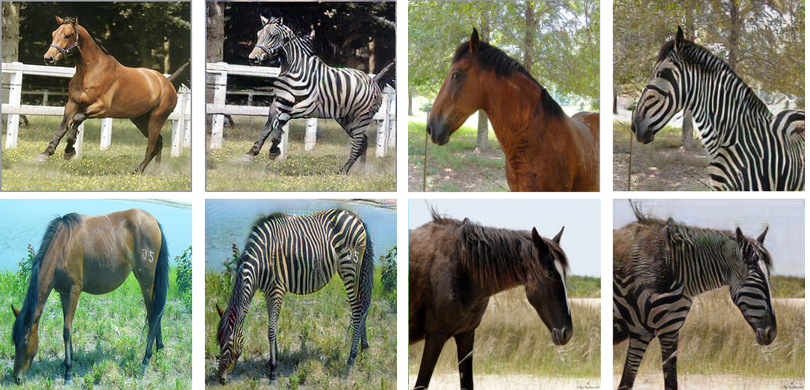
\includegraphics[width=1\columnwidth]{images/risultati cyclegan zebre.png}
\end{center}
\caption{Vediamo alcuni esempi di traduzione da cavallo a zebra dove la rete è riuscita a generare un'immagine accettabile.}
\label{fig:Risultati Cycle GAN base (1)}
\end{figure} 
Ovviamente la rete non è esente da difetti: in alcuni casi non riesce ad applicare uniformemente le strisce al manto del cavallo, rendendo evidente la falsità dell'immagine, oppure riconosce cavalli dove non ci sono, andando così a distorcere completamente l'immagine, come vediamo dagli esempi in figura \ref{fig:Risultati Errati Cycle GAN (1)} 

\begin{figure}[H]
\begin{center}
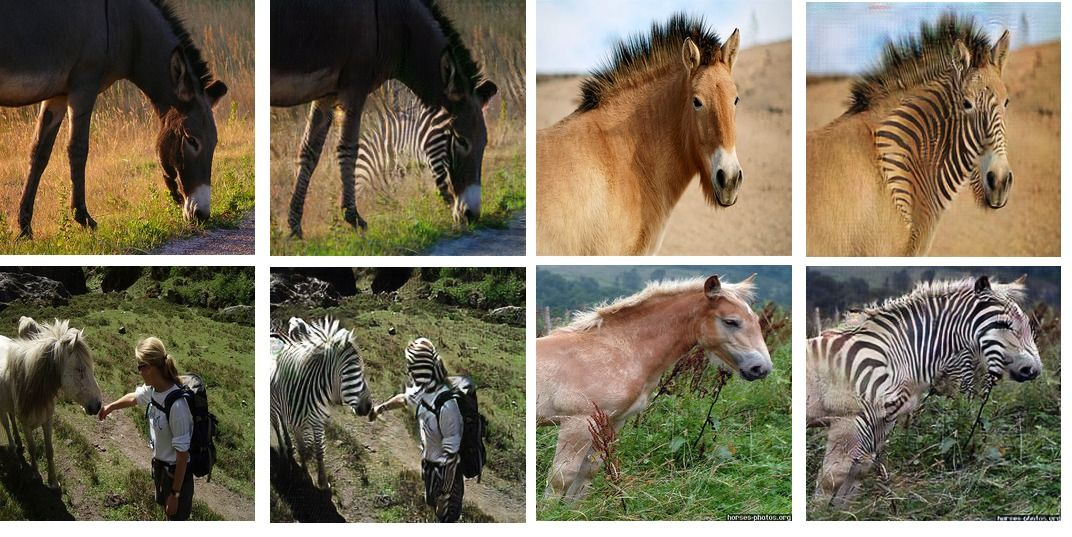
\includegraphics[width=1\columnwidth]{images/CycleGan zebre error.jpeg}
\end{center}
\caption{Vediamo come negli esempi di sinistra la rete non riesca a riconoscere il cavallo, mentre in quelli di destra la rete non riesca ad applicare le strisce in modo uniforme.}
\label{fig:Risultati Errati Cycle GAN (1)}
\end{figure} 

I risultati migliori sono quelli ottenuti da immagini in cui il cavallo è ben riconoscibile in foto e non è distante. La rete, inoltre, ha difficoltà a riconoscere la sagoma del cavallo quando nella foto sono presenti più cavalli, soprattutto se sovrapposti in prospettiva. L'algoritmo di FID applicato alle immagini delle zebre generate dalla rete, rispetto a tutte le immagini delle zebre del dataset, restituisce come risultato 33.66.
\subsection{Traduzione da zebre a cavalli}
Valutiamo ora la traduzione contraria, da zebre a cavalli. In questo caso, notiamo come la rete abbia più difficoltà nella generazione delle immagini, come vediamo in figura \ref{fig:Risultati Horse Cycle GAN (1)}. E' infatti difficile trovare tra i risultati immagini pienamente soddisfacenti, che mettano in difficoltà anche l'occhio umano, cosa che invece, nel caso precedente, accadeva con più frequenza.
\begin{figure}[H]
\begin{center}
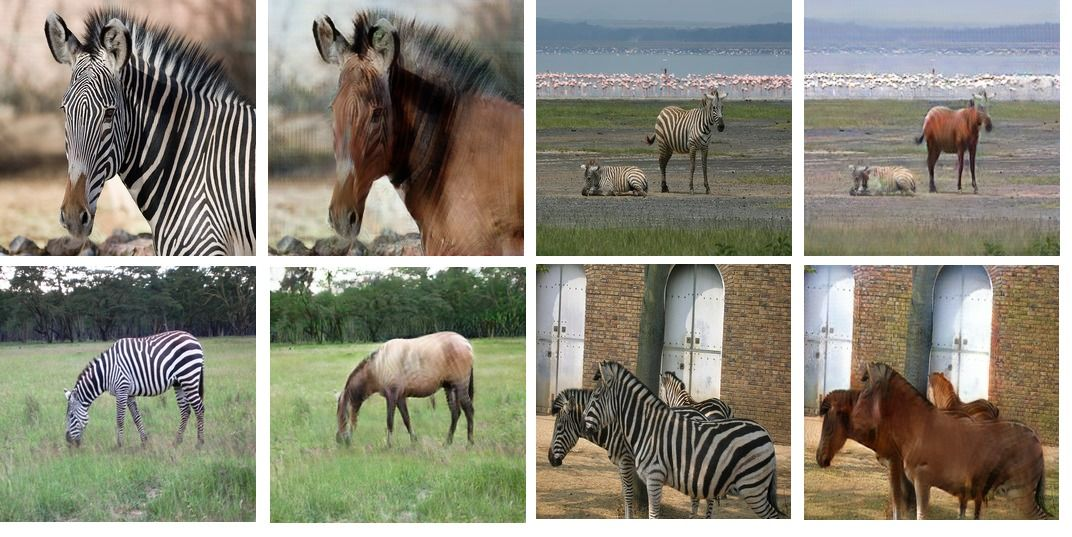
\includegraphics[width=1\columnwidth]{images/CycleGan horse (1).jpeg} 
\end{center}
\caption{Alcuni dei migliori risultati della traduzione da zebre a cavalli, vediamo come rimangano le strisce che la rete prova ad eliminare.}
\label{fig:Risultati Horse Cycle GAN (1)}
\end{figure} 
In questo caso l'algoritmo di FID, applicato rispetto a tutte le immagini dei cavalli presenti nel dataset, restituisce come risultato 64.57.

\section{Addestramento con trasferimento dell'attenzione}
Vediamo ora i risultati ottenuti dalla rete modificata utilizzando GradCam per generare la Loss di consistenza dell'attenzione. Sono stati effettuati più addestramenti con questa modalità, cambiando i parametri su cui ricavare l'attenzione, come vedremo successivamente. In questa sezione ci soffermeremo sui risultati ottenuti applicando il trasferimento dell'attenzione sull'ultimo blocco residuo. In questo caso, i risultati sono notevolmente migliorati nella traduzione da cavalli a zebre e hanno avuto un leggero miglioramento anche nella traduzione opposta.
\subsection{Traduzione da cavalli a zebre}
Come detto, si è migliorata l'efficienza della rete nella traduzione da cavalli a zebre. Infatti, i risultati mostrano una maggiore precisione nel riconoscimento del cavallo a cui applicare le strisce e una maggiore capacità di uniformare i cambiamenti. Come vediamo in figura \ref{fig:Risultati Zebre CycleGan + GradCam}, la rete genera, infatti, risultati migliori e più verosimili.
\\Ovviamente, anche in questo caso la rete non è perfetta, sono ancora presenti alcuni problemi nel riconoscimento dei cavalli in determinate foto, come ad esempio quelle ritraenti più cavalli distanti dall'obiettivo.

\begin{figure}[H]
\begin{center}
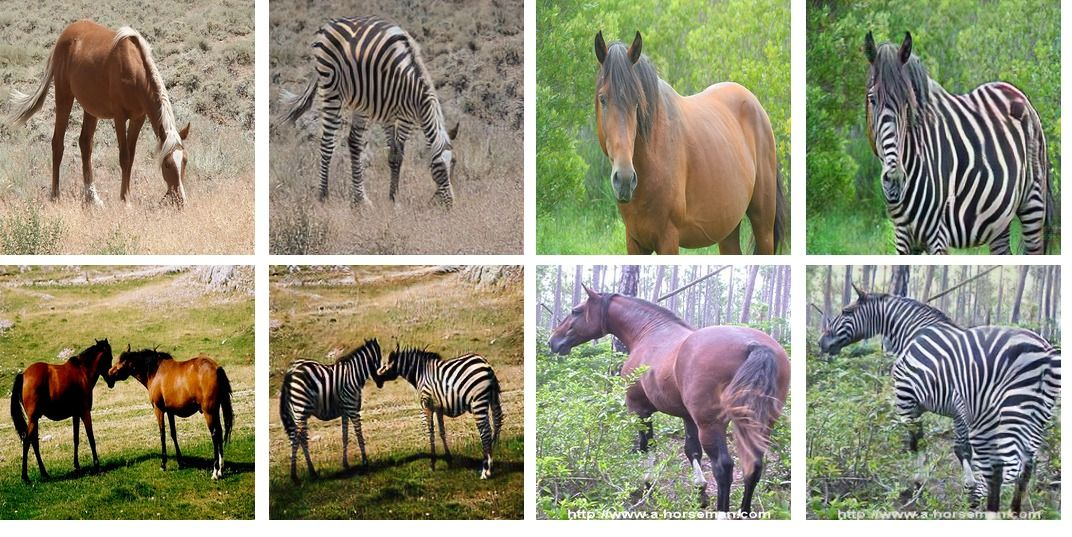
\includegraphics[width=1\columnwidth]{images/CycleGan + GradCam zebre.jpeg} 
\end{center}
\caption{Alcuni dei migliori risultati della traduzione da cavalli a zebre con trasferimento dell'attenzione, vediamo come le strisce siano più marcate ed uniformi.}
\label{fig:Risultati Zebre CycleGan + GradCam}
\end{figure} 

A sostegno di quanto affermato possiamo utilizzare l'algoritmo di FID ottenendo un risultato di 27.9.

\subsection{Traduzione da zebre a cavalli}
Come affermato precedentemente, in questo caso il miglioramento è minimo. Infatti, la rete fa ancora fatica ad eliminare uniformemente le strisce bianche e nere delle zebre, come vediamo dalla figura \ref{fig:Risultati cavalli GradCam}. I risultati sono molto simili ai precedenti, lo dimostra anche il risultato del FID, pari a 61.5, ancora molto elevato.
\begin{figure}[H]
\begin{center}
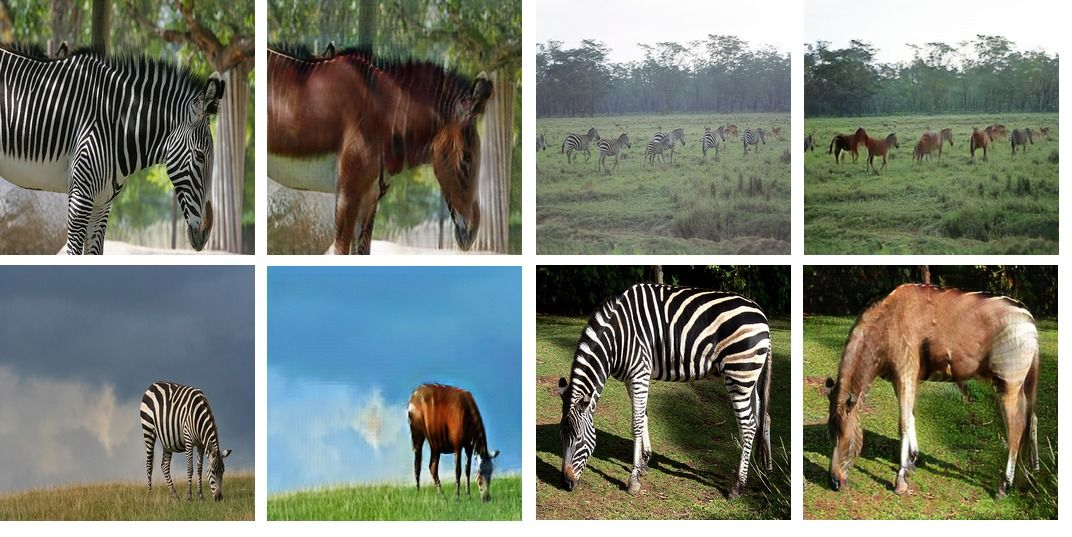
\includegraphics[width=1\columnwidth]{images/image (2).jpeg} 
\end{center}
\caption{Alcuni dei migliori risultati della traduzione da zebre a cavalli, vediamo come, anche in questo caso, rimangano le strisce che la rete prova ad eliminare.}
\label{fig:Risultati cavalli GradCam}
\end{figure} 

\section{Confronto tra le due reti}
Abbiamo dunque visto come la rete venga migliorata applicando il trasferimento dell'attenzione. Ora possiamo andare nel dettaglio e, aiutandoci tramite esempi generati da entrambe le reti, confrontare i risultati.
\\\emph{Per comodità le reti verranno da qui in poi indicate come rete \emph{standard} e rete \emph{GradCam}}
\\Nella sezione precedente, avevamo indicato tra i problemi della rete \emph{standard} la difficoltà nell'applicare in maniera uniforme le strisce bianche e nere ai cavalli; questo problema, come vediamo in figura \ref{fig:Confronto GradCam e noGradCam}, viene perfettamente risolto dalla rete \emph{GradCam}. Inoltre, le immagini generate dalla rete \emph{GradCam} hanno mediamente una qualità migliore rispetto alle altre. Questo lo si nota andando ad analizzare lo sfondo delle immagini generate: nel caso \emph{standard}, molto spesso, esso risultava essere corrotto, oppure perdeva colore, risultando la maggior parte delle volte più scuro e opaco. Nel caso della rete \emph{GradCam}, invece, lo sfondo risente meno di questi peggioramenti, come notiamo dal colore del cielo della prima immagine della figura \ref{fig:Confronto GradCam e noGradCam}, e ciò porta ad una migliore qualità nel complesso. La rete \emph{GradCam} è inoltre in grado di riconoscere meglio i cavalli: infatti alcuni di essi, specie quelli dal manto completamente nero, mettevano in seria difficoltà la rete \emph{standard}, mentre la rete \emph{GradCam}, seppur non ancora in maniera ottimale, riesce a portare buoni risultati anche su questa tipologia di immagini.
Un ulteriore miglioramento che salta all'occhio risiede nel colore del manto delle zebre generate dalla rete \emph{GradCam}: molto spesso infatti, anche nelle migliori immagini generate dalla rete \emph{standard}, il manto presentava sfumature scure, tendenti al marrone, dovute al colore del cavallo originale. Nelle immagini prodotte dalla rete \emph{GradCam}, invece, queste sfumature si sono, nella maggior parte delle immagini, azzerate.



\begin{figure}[H]
\begin{center}
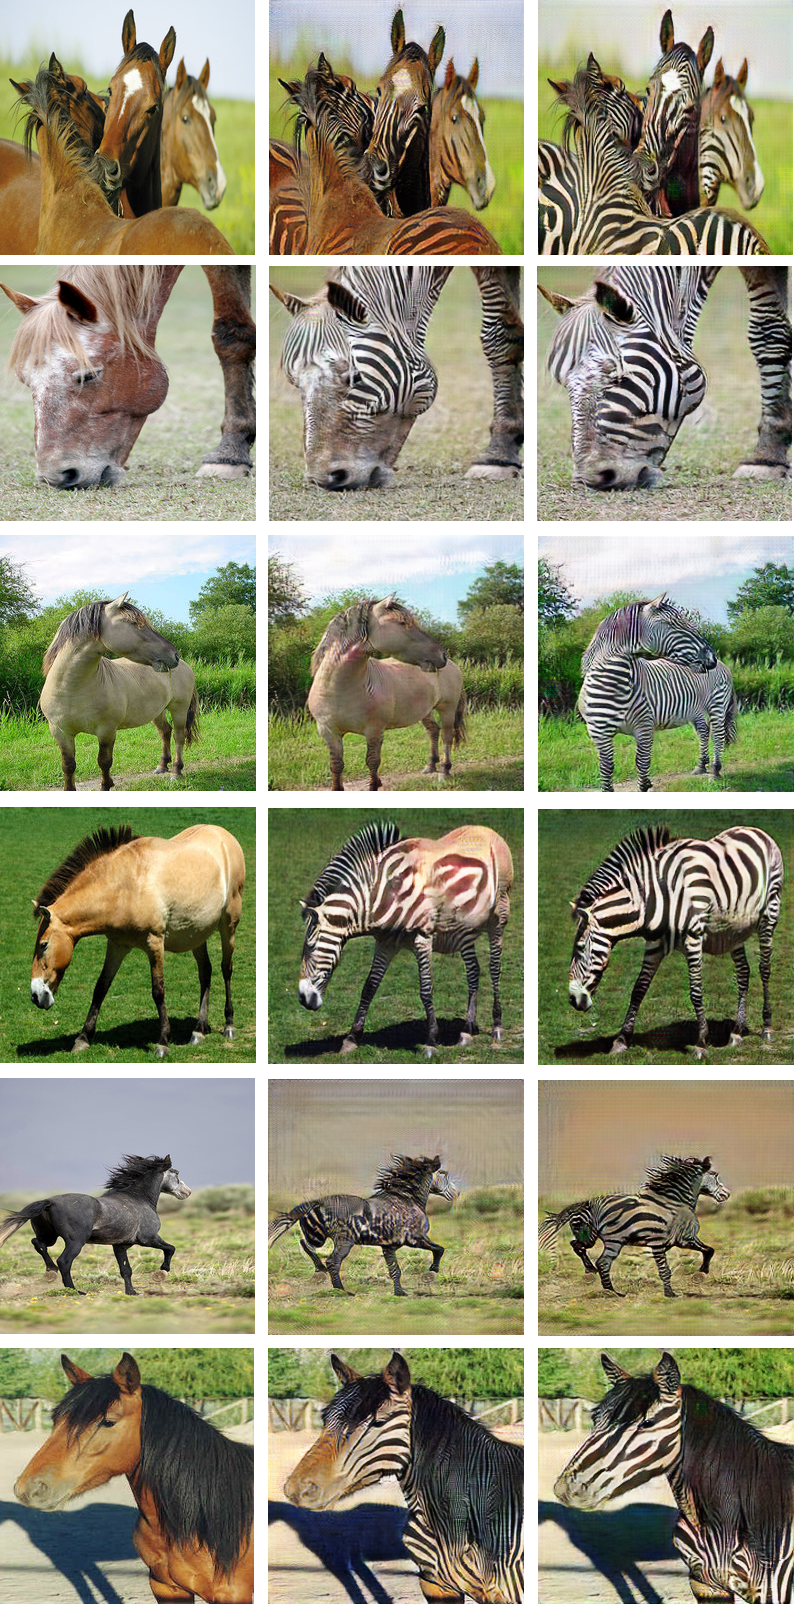
\includegraphics[width=0.6\columnwidth]{images/merge zebre.png}
\end{center}
\caption{In foto il confronto tra immagine reale, immagine generata senza GradCam e immagine generata dalla rete con GradCam.}
\label{fig:Confronto GradCam e noGradCam}
\end{figure}  
Un discorso simile lo si può fare anche trattando la traduzione da zebre a cavalli: infatti, seppur i risultati siano ancora lontani dalla realtà, possiamo notare alcuni miglioramenti. Come vediamo in figura \ref{fig:Confronto GradCam e noGradCam cavalli}, la rete \emph{GradCam} si dimostra migliore nell'eliminazione delle strisce bianche e nere, specie in quelle immagini che ritraggono le zebre in primo piano. 
\\Nonostante questi miglioramenti, rimane però il problema principale che caratterizzava la rete \emph{standard}: non si riescono ad eliminare perfettamente le strisce delle zebre. Entrambe le reti, infatti, non mostrano particolare difficoltà nel differenziare l'animale dallo sfondo, cosa che accade nella traduzione opposta, ma hanno elevata difficoltà nell'eliminazione delle strisce bianche e nere, tant'è che la maggior parte dei risultati presenta ancora strascichi delle strisce, come vediamo dalla figura \ref{fig:Confronto GradCam e noGradCam cavalli}.


\begin{figure}[H]
\begin{center}
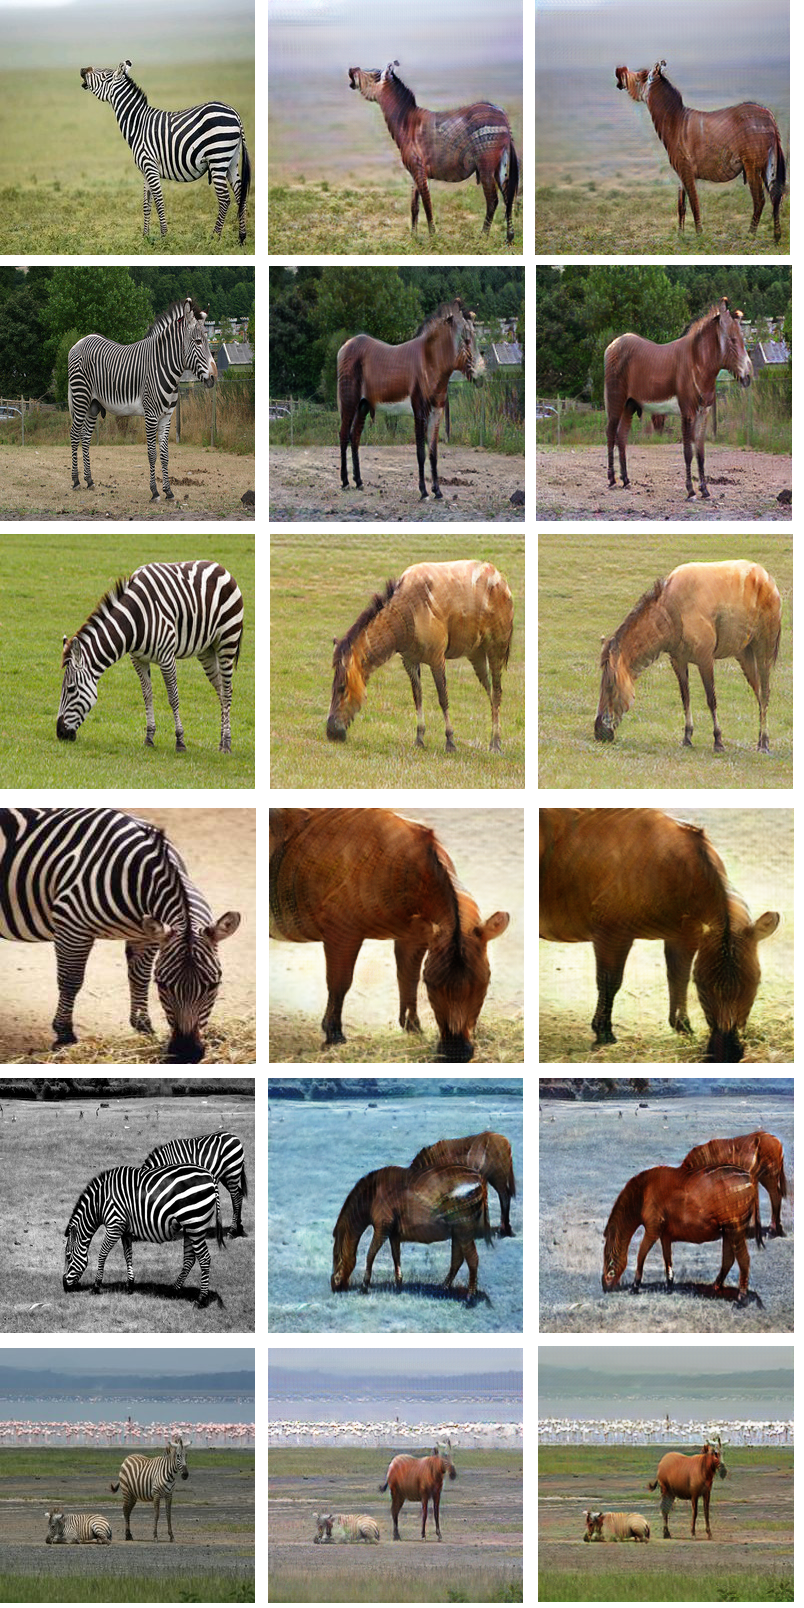
\includegraphics[width=0.6\columnwidth]{images/merge.png}
\end{center}
\caption{In foto il confronto tra immagine reale, immagine generata senza GradCam e immagine generata dalla rete con GradCam.}
\label{fig:Confronto GradCam e noGradCam cavalli}
\end{figure}  

\section{Ulteriori sviluppi per la rete}
Dopo aver commentato i risultati ottenuti sfruttando GradCam sull'ultimo blocco residuo ed averli confrontati con i risultati della rete \emph{standard}, possiamo ora analizzare le ulteriori modifiche che abbiamo apportato alla rete. Infatti, al fine di migliorare i risultati ottenuti, abbiamo provato a modificare alcuni parametri della rete, sempre utilizzando l'algoritmo GradCam. Prima di entrare nel dettaglio, è bene specificare che tra tutte le reti provate, quella migliore, basandoci sul risultato dell'algoritmo FID, rimane la rete \emph{GradCam}, come vediamo dalla tabella \ref{tab:Fid Table}.
\\Le modifiche apportate alla rete sono state le seguenti:
\begin{itemize}
\item Utilizzo di un coefficiente pari a 0.1 per la Loss di consistenza dell'attenzione;
\item Utilizzo di GradCam solo nella traduzione \emph{primaria}, quindi solo da dal dominio $A$ al dominio $B$;
\item Utilizzo di GradCam attraverso un \emph{detach} sulle immagini fake generate per il calcolo della Loss;
\item Utilizzo di GradCam su quattro blocchi residui.
\end{itemize}



\begin{center}
\begin{tabular}{ | c | c | c | }
\hline
\textbf{Rete}          & \textbf{FID Zebre}        &   \textbf{FID Cavalli}    \\
\hline
\emph{standard}          & 33.66     & 64.57  \\ \hline
\emph{GradCam}           & 27.94     & 61.54  \\ \hline
\emph{GradCamWithCoeff}  & 31.90     & 66.01  \\ \hline
\emph{GradCamA2B}        & 30.60     & 65.32  \\ \hline
\emph{GradCamWithDetach} & 32.74     & 62.71  \\ \hline
\emph{GradCamFourLayers}   & 33.18     & 61.77  \\ \hline
\end{tabular}
\captionof{table}{Comparazioni tra i valori dei FID delle varie architetture utilizzate.}
\label{tab:Fid Table}
\end{center}

Andando più nel dettaglio vediamo perchè abbiamo provato queste modifiche alla rete.
\\Per quanto riguarda il coefficiente applicato alla Loss di consistenza dell'attenzione, abbiamo ragionato sul fatto che, senza questo coefficiente, la Loss sarebbe potuta essere troppo elevata rispetto alle altre presenti all'interno della rete, e, per questo motivo, avrebbe potuto sbilanciare il calcolo più in suo favore, riducendo i contributi delle altre Loss.
\\Il ragionamento che ci ha spinti, invece, ad utilizzare GradCam solo per la traduzione da $A$ a $B$ invece è dovuto al fatto di voler provare ad utilizzare il trasferimento dell'attenzione solo per la traduzione da cavalli a zebre, in quanto è in questa traduzione che si riscontrano i risultati migliori.
\\L'utilizzo del \emph{detach} sulle immagini fake durante il calcolo della Loss, di cui vediamo il codice:
\begin{minted}[bgcolor= lightGray]{Python}
self.att_lossA2B = self.MSE_LOSS(self.cam_fake_B.detach(),
                             self.cam_rec_A)
self.att_lossB2A = self.MSE_LOSS(self.cam_fake_A.detach(),
                             self.cam_rec_B)
\end{minted}
è stato fatto perchè senza di esso sono entrambe le attenzioni che tendono ad un'attenzione comune, sia quella dell'immagine reale che quella dell'immagine fake. Idealmente, però, sarebbe solo l'attenzione dell'immagine fake a doversi adattare a quella dell'immagine reale, ed è proprio a questo che serve il \emph{detach} posto prima del calcolo della Loss.
\\Infine, l'utilizzo di GradCam su quattro blocchi residui, anzichè solo sull'ultimo, è stato effettuato per provare a migliorare la consistenza dell'attenzione. I layer scelti (10,14,15,18), infatti, mostravano i risultati migliori nella generazione delle attenzioni.
Concludiamo questa sezione andando a vedere i risultati generati dalle varie reti sulle stesse immagini. Come vediamo dalle figure \ref{fig:Confronto tra tutte le reti zebre} \ref{fig:Confronto tra tutte le reti cavalli}, la rete \emph{GradCam} si conferma la migliore.


\begin{figure}[H]
\begin{center}
\includegraphics[width=1\columnwidth]{images/allOrdine.png}
\end{center}
\caption{In foto il confronto tra le immagini generate dalle reti, ordinate decrescentemente da sinistra a destra secondo il risultato dell'algoritmo di FID.}
\label{fig:Confronto tra tutte le reti zebre}
\end{figure}  

\begin{figure}[H]
\begin{center}
\includegraphics[width=1\columnwidth]{images/All Cavalli.png}
\end{center}
\caption{In foto il confronto tra le immagini generate dalle reti, ordinate decrescentemente da sinistra a destra secondo il risultato dell'algoritmo di FID.}
\label{fig:Confronto tra tutte le reti cavalli}
\end{figure}  

\clearpage

          \chapter{Conclusioni e sviluppi futuri}
In questo capitolo finale tratteremo i possibili sviluppi futuri che possono essere apportati al sistema realizzato, al fine di migliorarne le prestazioni sia in termini di risultati, sia in termini di efficienza del codice.

\section{Conclusioni}
Prima di procedere illustrando i possibili sviluppi della rete è bene ricapitolare brevemente le conclusioni dedotte dai risultati commentati nei capitoli precedenti.
\\Come prima cosa, la più importante, possiamo dire di aver ottenuto dei risultati pienamente soddisfacenti. Lo scopo del sistema, infatti, era quello di migliorare la CycleGan proposta dal Paper \cite{Zhu_2017_ICCV} grazie al trasferimento dell'attenzione durante l'addestramento. Scopo che, come ampiamente trattato nel capitolo precedente, è stato portato a termine. Abbiamo visto, infatti, come i risultati della rete che sfrutta GradCam sull'ultimo blocco residuo siano migliori rispetto alla rete \emph{standard}. Abbiamo ottenuto dei risultati migliori applicando GradCam su entrambi i dataset utilizzati. 

\clearpage

\appendix
\renewcommand{\chaptermark}[1]{\markboth{{\appendixname}\ \thechapter.\hspace{1em}#1}{}}

\chapter{Appendice}



\clearpage

\addcontentsline{toc}{chapter}{Bibliografia}
\bibliographystyle{unsrt}
\nocite{*}
\bibliography{riferimenti}
% 
\clearpage

\end{document}


